% !TeX spellcheck = en_US
\documentclass[11pt,a4paper,twocolumn]{book}
\usepackage[latin1]{inputenc}
\usepackage{amsmath}
\usepackage{amsfonts}
\usepackage{amssymb}
\usepackage{graphicx}
\usepackage[table]{xcolor}
\usepackage{wrapfig}
\usepackage{multicol}
\usepackage{multirow}
\usepackage{paralist}
\usepackage{longtable}
\usepackage{tabu}
\usepackage{soul}
\usepackage{titling}
\usepackage{pdfpages}
\usepackage[hidelinks]{hyperref}

\hypersetup{
	colorlinks,
	citecolor=black,
	filecolor=black,
	linkcolor=black,
	urlcolor=black
}

\title{Wanderers' Files}
\date{\today} 

\begin{document}
	
	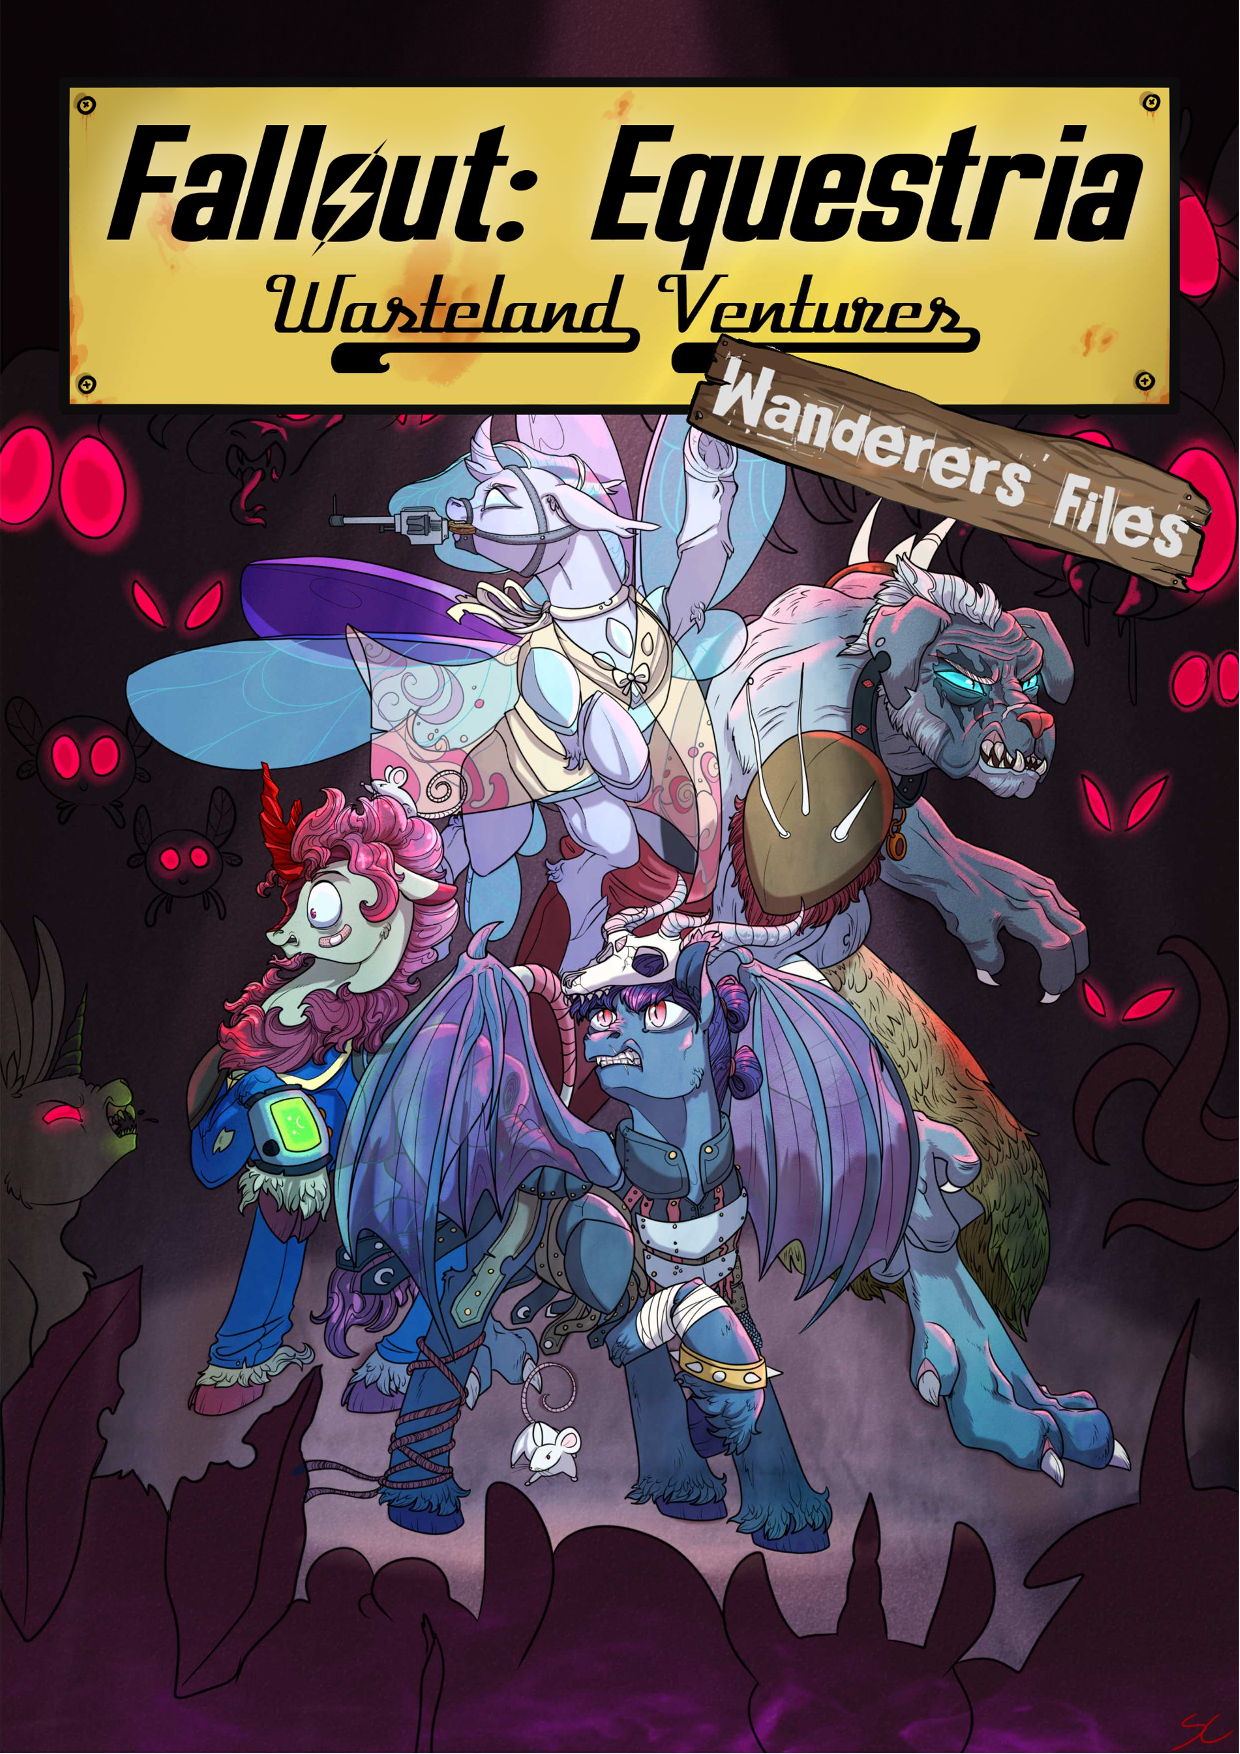
\includepdf[pages={1}]{WORD/COVER-WANDFILE.pdf}		
	\onecolumn
	\setcounter{page}{1}	
	\begin{center}
		Compiled by Waak, Kireanikin, LaPa, Miksu \& SourCherry
		
		10 AP rule basis by Yondalor
		
		Token HP \& Status rule bases by LZ
		
		\bigskip		
		\textbf{Playtesting and Advice:} LZ, Moonlight, Mittens, Kittyfluff, Ray\_Lionheart, f1r3w4rr10r, Tierney Kelly, Eden, Kendallkun, Pesian, Raven, dumbhat, GODOG, Borealis
		
		\bigskip
		\textbf{Cover and Graphics:} SourCherry
		
		\bigskip
		\textbf{Layout:} Waak \& SourCherry		

	\end{center}
	
	\vfill
	
	\begin{center}
		\textbf{Version 1.4.1}
		
		\emph{Last compiled on \thedate}
        
        \emph{\textbf{Contact:} wasteland-ventures@googlegroups.com}
     
	\end{center}	
    \begin{figure*}[bp]
		\centering
		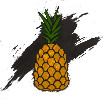
\includegraphics[width=3cm]{ART/ISA_Logo}
	\end{figure*}

	\twocolumn
	\tableofcontents


	\chapter{Introduction}
	
	The purpose of this book is to introduce new playable races into the system and everything they need to function, including their own brands of magic if applicable. In addition, the book holds in it the core races for the sake of having the full roster of playable characters present.
	
	The new magic systems were made to make some of the races a bit more unique and interesting.
	
	\chapter{Races}
	
	It wasn?t only ponies, zebras and griffons who survived the horrors of the apocalypse and t

	\section*{Abyssinian}
	\addcontentsline{toc}{section}{Abyssinian}
	A race of bipedal cats, abyssinians hail from a kingdom outside of Equestria?s borders. Hence why this race is rarely seen in the Wastes, as not many were present during the Last Day. However, while Equestria is now little more than a dead wasteland, Abyssinia has thrived, building their nation further. Yet, perhaps compelled by the feline curiosity, some make their way to the Equestrian Wasteland... 
	
	Though food and shelter is plenty in Abyssinia, the various magitech constructs they developed during the war are scarce and in bad shape, due to Abyssinia being low in magic-amplifying gems, which the Equestrian Wasteland still has in droves.
	
	Being feline in origin, abyssinians have the smooth, graceful moves of a cat, often bending and moving in ways ponies cannot. In addition to this, they have sharp claws on their paws that they can and often use to fend for themselves, and, much like bat ponies, abyssinians have slit pupils, and can see much better in dark than most equine species.
	
	The witches? black cats know tricks, as abyssinians wield magic like Unicorns. Their bodies and minds are also more adapted to magic, having greater resistance to arcane fatigue. 
	Instead of having a horn like the equine spellcasters, abyssinians use trinkets, wands and staffs to focus the magical energies they harness. Though abyssinians can cast magic without a catalyst -a magical artifact unique to each caster-, their delivery of the spell weakens considerably. 
	Traditionally, each abyssinian mage crafts their own catalyst, as it is believed that this allows the mage to channel their magic best. These catalysts are considered to reflect the mage?s virtue and personality. Should the catalyst break, they have to craft a new one (Thaumaturgy roll) with materials they feel reflect their personality the most.
	
	Abyssinians have the following racial abilities:
	\begin{description}
		\item[Eye in the Dark:] Abyssinians' eyes are made for hunting in the dark, letting them ignore 10 points of Visibility penalty caused by dark surroundings.
		\item[Sorcerer:] Abyssinians can tap into the same magical energy as unicorns do, giving them access to Unicorn Magic. Abyssinians can choose 3 Unicorn spells at character creation, and they have additional 10 Strain. However, they cannot learn new spells by level-up. They can only learn new spells by studying.
		\item[Cat-Alyst Caster:] Abyssinians perform their spellcraft through magical catalysts, such as wands, staffs, trinkets and jewelry. Abyssinians craft these artifacts from various mutant parts and junk. Casting spells without said catalyst removes the SPECIAL bonus from their spells? Potency, and adds +1 Strain cost.
		\item[Predator:] Abyssinians possess natural claws, giving them an extra dice to damage when using bare paws as Unarmed weapons.
	\end{description}
	
	\clearpage
	
	\section*{Bat Pony}
	\addcontentsline{toc}{section}{Bat Pony}	
	Bat ponies, though possessing same flight capabilities as pegasi, are otherwise a distinct race of their own. Most remaining tribes of bat ponies have kept to their ancestral homes deep in the cavernous Equestrian mountains. However, the Enclave and several mutated cave-dwellers have forced some tribes to come into view, so to speak.
	
	Some of the bat ponies were employed by Princess Luna as her personal guard and chariot-pullers. Perhaps due to both Princess Luna?s influence and their isolation from much of the Wasteland, the bat ponies? speak can sometimes sound archaic, though many do make a conscious effort to leave this habit into the past.
	
	Equipped with leathery bat wings -hence the name- and slit pupils, bat ponies are further divided from the other pony brethren by their relatively subdued and neutral color schemes of their mane and coat, though exceptions have been known to happen.
	
	Bat ponies? eyes react to light much like any dark-dwelling creature?s would, outwardly seeming quite cat-like, with their pupil changing size depending on amount of light the eye detects. Due to this, they have an excellent dark-vision, but color vision is quite poor.
	
	Bat ponies have the following racial abilities:
	\begin{description}
		\item[Cutie Mark:] Bat ponies have a special talent, giving them +5 to a skill when using their special talent.
		\item[Friend of the Night:] Bat ponies' eyes are well-versed for traversing in the dark, letting them ignore 10 points of Visibility penalty caused by dark surroundings.
		\item[Leathery Wings:] Bat ponies have wings and can fly. They can increase their flight capabilities by investing in Aerial Maneuvers.
		\item[Night Flight:] Bat ponies have a limited ability to perform Aerial Maneuvers. They can choose 2 at 1st level they have the requirements for, and gain a new one every 6 levels after (7th, 13th...). They have access to Wonderbolt Maneuvers.
	\end{description}

	\clearpage
	
	\section*{Brahmin}
	\addcontentsline{toc}{section}{Brahmin}
	
	Brahmin are the descendants of the mutated cows and bulls of wartime Equestria, most notable of their features being their two heads. As brahmin can be -though it is a rather rare instance- sentient, they often wear armor to protect themselves. And perhaps due to their large size and strong physique, they are excellent at hauling heavy weights.
	
	Out of the two heads brahmin possesses only one of the heads is sentient, the other has devolved to be little more than an animal working on instinct. Sometimes, the non-developed head can act on its own, but rarely does much harm on purpose.
	
	Though brahmin cows are more common sight in the Equestrian Wasteland, brahmin bulls also exist. Aside from lacking female brahmin?s bloated udders, they are similar in general appearance, only larger and perhaps a bit more hearty in stature. Both genders have horns, often in mismatched places, that continue to grow all throughout the brahmin?s life.
	
	Brahmin, much like the wartime cows and bulls, get along well with ponies, usually finding their stay in pony-centered cities leisurely and accommodated, even if it is technically a livestock stable...
	
	Brahmin have the following racial abilities:
	\begin{description}
		\item[Big Betsy:] Brahmin are able to pull heavier loads than most other species, and due to this, they do not suffer Encumbered-status from Heavy Armor that weight 15 kg or less.
		\item[Easy Load:] Brahmin have strong back, letting them carry much more than a pony could. Brahmin have +20 kg to their Carry Weight limit.
		\item[Fresh Pair of Eyes:] With additional head, brahmin are harder to surprise. They gain +10 to PER rolls against Stealth. However, the additional head comes at a price, being another Head that can be Crippled - thus brahmin may suffer from two Crippled heads, and their cumulative penalties.
	\end{description}
   
   	\clearpage
   	
   	\section*{Buffalo}
   	\addcontentsline{toc}{section}{Buffalo}
   
  	 Buffalo are the offspring of the tribals that roamed the southernmost plains and arid ranges of Equestria, especially around the old towns of Appleloosa and Dodge Junction. 
   
  	 Still holding tradition close to their hearts, buffalo maintain their identity strongly through their customs, such as an annual roam through a specific route in the mid-west Equestria, that has been roamed for countless generations. This adherence to tradition is still seen as odd in eyes of ponies, but most buffalo would agree that tradition makes them stronger and creates unity in a tribe.
   
   	Shamanism is strong with buffalo, being the only other race to communicate with spirits on a regular basis alongside zebra. Much like with zebra, this gift is highly respected in their communities as though many buffalo see and interact with spirits daily, but only a proper shaman can barter with them. Buffalo Shamans are often high in the social order, being the one to link the buffalo to their ancestry and to the nature around them and to give advice to the community by spirit counseling.
   
   	\textbf{Buffalo may take Shaman perks, if they possess Tribal Shaman trait.}
   
   	Buffalo have the following racial Abilities:
   	\begin{description}
	   	\item[Tribal Ancestry:] Buffalo, much like zebra, have a long history of shamanism in their tribes, with shamans holding much power and reverence. Buffalo have access to Spirit Magic and Tribal Shaman trait.
	   	\item[Easy Load:] Buffalo have strong back, letting them carry much more than a pony could. Buffalo have +20 kg to their Carry Weight limit.
	   	\item[Great Beast:] Buffalo are visibly larger than ponies, and have heavier builds. All buffalo are considered to be Size Category 1 at start, and they also gain an extra SPECIAL point to invest during character creation.
	   	\item[Healer:] Buffalo have a long history with medicine, from herbal mixtures to high-end chemistry. With a careful dosage, they can administer a Medical item twice, excluding  Doctor?s Bag and First Aid -kit.
	\end{description}

	\clearpage
	
	\section*{Changeling}
	\addcontentsline{toc}{section}{Changeling}
	
	One of the more evasive races in the Equestrian Wasteland, the changelings are shapeshifters whose original form resembles a thin insect and pony hybrid. Commonly seen as Equestria?s version of the boogeyman, due to their transformative magic hiding them in plain sight, many independent hives began to break out of their old molds after the Last Day; some for the better, some for the worse. Most settlements in Wasteland regard changelings with suspicion and fear, though there are exceptions.
	
	Changelings are unique in that they do not get the bulk of their nutrients from regular food -though eating material things is still somewhat useful during a shortage-, but rather they gather and eat emotions (Strain in this system) from ponies. To successfully steal emotions from them, they take the form of the pony?s loved one and feed off of the pony?s affections for that person. This is often preceded by getting rid of the original... 
	
	However, changelings are not perfect copies of the pony they?re posing as, only of their outward appearance, leaving their behavior something that a changeling has to study well to not get caught.
	
	Changeling hives rarely have contact with one another, causing a large chasm of differences from hive to hive, from their tactics to gather energy, to their general opinion on other creatures and to customs regarding social standing and cultural customs. Most commonly, the hive is ran by a changeling queen, a taller and more powerful creature than the common changeling. She makes the decisions in the hive, with or without input from her subjects. 
	
	Though changelings themselves have life-span of an average pony, the changeling queen can live hundreds of years, meaning that some of the changeling queens are old enough to remember the war and its cause and effect.
	
	Changelings have the following racial abilities:
	\begin{description}
		\item[Changeling Magic:] Changelings have a magic that is a mixture of Unicorn magic schools and their own unique spells. See Changeling Magic for details. Changelings start with Shapeshift for free, and 3 additional spells. They learn a new spell every 5 levels (6th, 11th...).
		\item[Contort:] Changelings have bug-like qualities, and they can contort their bodies in ways ponies cannot. They have +10 to Unarmed when grappling.
		\item[Strain Feeder:] Changelings feed off Strain of others because they do not regenerate Strain on their own. Strain can be given to the changeling willingly, or taken by force. See Changeling Magic for more details.
		\item[Chitinous Shell:] Changelings have thick chitin that gives them armor-like properties. This provides +5 DT when not wearing Heavy or Power armor.
	\end{description}
	
	\clearpage
	
	\section*{Crystal Pony}
	\addcontentsline{toc}{section}{Crystal Pony}
	
	Crystal ponies resemble earth ponies in outward appearance, but their shiny, crystal-like coat and gradiented manes set them apart from their earthy cousins. Hailing from the northern Crystal Empire, these ponies remained impartial to the conflict of the warring Equestria, though it was rumored that the empire was assisting them under the table, so to speak.
	
	The Crystal Empire?s ample defenses ensured that the stray bomb that hit near Yakyakistan would not cause as much harm on them as it did on the yaks, as the force field surrounding the empire kept much of the radiation at bay. However, the shield did not stop all of the magical fallout and the nuclear winter it brought with it from seeping in. For the first half a century, the Crystal Empire skies were sunny and the climate warm and the only sign of adversity were from an occasional feral ghoul here and there. 
	
	But soon it was found out that the power of the Crystal Heart was dwindling, allowing for more and more radiation to seep in, and the environment to grow colder. Emergency measures were taken to power the Crystal Heart, but they ultimately proved futile. As the radiation and nuclear winter engulfed the city, the crystal ponies found themselves with an empire unable to sustain itself properly. Despite this, the Crystal Empire still has some few stubborn individuals remaining to this day.
	
	Crystal ponies have the following racial abilities:
	\begin{description}
		\item[Cutie Mark:] Crystal ponies have a Special Talent, giving them +5 to a skill when using their special talent.
		\item[One with the Glow:] Though balefire is not the source of their mutation -that would be the Crystal Heart, an ancient magical artifact that gave off magical radiation much like a prototype megaspell-, crystal ponies are considered mutated. Due to this they have a boosted Poison Resistance of 15 and Radiation resistance of 10.
		\item[Abhorrent Past:] Crystal ponies are more in tune with their emotions, and this, coupled with the tyranny they suffered under king Sombra, has left them less capable of dealing with hardship. Their Insanity Chance is 25\% instead of 20\%. However, they did survive the tyranny and came back stronger: They have +1 to END to resist Mind-Control -status effect.
		\item[Ties to the Earth:] Much like their earth pony cousins, crystal ponies share their connection to earth. This gives them access to Earth Pony magic, and start with 3 Spells and gain a new one every 6 levels after (7th, 13th...).
	\end{description}

	\clearpage
	
	\section*{Deer}
	\addcontentsline{toc}{section}{Deer}
	
	Deer used to inhabit many of the Equestrian forests with their own kingdoms. Rather a  rare sight, as most ponies are used to seeing the deer?s unfortunate mutation, the Radstag. However, despite the popular notion that sane deer didn?t make it out of the magical fallout, some of the population did survive in a bunker of their own making.
	
	As the decades rolled on and the once lush forests either grew too hostile or died, the deer can sometimes be spotted in settlements surrounding their abandoned and overtaken kingdoms. However, the deer are still ruled by their community?s king, which is a hereditary position, unless the heir is too young or unfit to rule. 
	
	Outwardly, the deer are tall and lithe, their movements graceful and cautious. Around their necks, deer carry a cask, that can vary in shape and size. This cask contains a potion of their own making. However, unlike ponies, deer fare worse against the magical fallout, and due to this one can often find deer wearing a breather of sorts to protect their lungs from irradiated air.
	
	Deer?s Cask functions as a Quick Slot.
	
	Deer have the following racial abilities:
	\begin{description}
		\item[Blessing of the Green:] Deer utilize their magic with potions made from plants and earth from their surroundings, much like how zebra use alchemy to brew their potions. They have access to the Alchemy list, and start with 4 recipes with Skill Requirement of 30 or less.
		\item[Purity Flaw:] Deer are less tolerant of magical radiation and often require breathers to steer clear of harmful effects. Their Poison resistance is 15 and their Rad resistance is 0. However, they recover from wounds better than most races; they have +1 to Natural Healing Rate.
		\item[Quick Runner:] Deer are quick and agile creatures, reacting quickly to events happening around them, even when surprised. They have +2 to Initiative.
		\item[Sharp Horns:] Deer possess branching horns, giving them an extra die to damage when using horns as Unarmed weapons.
	\end{description}

	\clearpage
	
	\section*{Diamond Dog}
	\addcontentsline{toc}{section}{Diamond Dog}
	
	Though many diamond dogs have mutated into the fearsome hellhounds, some packs have eluded this fate. Retaining their form largely unchanged, diamond dogs are canine creatures that can walk on both four legs or two, giving them ample choices for weaponry.
	Diamond dogs have keen sense of smell and hearing, Much like their name implies, they have a great greed for gemstones. Due to this, they mostly inhabit caves and caverns, with strict hierarchy -a trait that remained in the mutated hellhounds- defining their way of life.
	
	Most packs of diamond dogs are led by an alpha, or if the alpha has deceased, by their companion, the matriarch. The alpha and matriarch both have a high social standing, with the alpha upholding and planning daily hunts, digs and gem hauls, as well as having the final say on who does what. The matriarch makes sure the community works well together, negotiating and separating individuals in a fight; she also handles issues in pup-caring. Much like pony societies, these packs can have good and bad leaders, resulting in vastly different packs. 
	
	However, despite their strict social hierarchy, members are free to roam if they want to, and can rise up in ranks through recognition as a valuable member. More often than not, the higher the rank, the more gemstones the diamond dog has on them. 
	
	Due to the wartime stories -of the second class citizenship diamond dogs had to endure in Equestria- that mothers pass on to their pups, diamond dogs do not mingle well with ponies; they are usually cautious and wary of any pony, and take a while to warm up to them. Other races however, rarely encounter this cautious behavior.
	
	Diamond dogs have long, thick claws that are primarily used for digging, and though they are not quite as strong and sharp as hellhound?s, they can dig through most common rock material and soil. They can also see fairly well in dark, though not quite as well as bat ponies or abyssinians. Diamond dogs are capable of eating plant material, but prefer fresh meat vastly over vegetables.
	
	Diamond Dogs have the following racial abilities:
	\begin{description}
		\item[Canine Claws:] Diamond dogs possess natural claws, giving them an extra die to damage when using bare paws as Unarmed weapons. In addition, said claws can pierce through meager armor, ignoring 5 DT.
		\item[Accustomed to Dark:] Diamond dogs? eyes are made for roaming their underground lairs, letting them ignore 5 points of Visibility penalty caused by dark surroundings.
		\item[All Ears:] Diamond dogs have sharp hearing, giving them +1 to PER when locating sneaking enemies, and +2 to Initiative. However, said hearing is sensitive to high-pitched sounds, giving them Moderate Distraction whenever subject to them. This includes whining from pony mares.
		\item[Underground Dweller:] Due to their habitat being self-dug caves and caverns, diamond dogs can ignore Difficult Terrain when traveling underground.
	\end{description}

	\clearpage
	
	\section*{Donkey}
	\addcontentsline{toc}{section}{Donkey}
	
	Though they?re hardly the next beauty queen winner, or even the runner-up, donkeys do have their place in the Equestrian Wasteland. Due to their sturdy nature, they?ve fared quite well despite the magical fallout. 
	
	Unlike ponies and various other magical creatures, donkeys are inherently magicless, making up for it with their tenacity and stubborn determination to see that their goals succeed. Donkey culture doesn?t vary much from pony culture, which is why donkeys often assimilate to society easily. 
	The only key difference is the donkey societies? more inward approach to strangers, not being quite as eager to befriend as ponies are. This usually means they?re slow to warm up to others they do not know well, but once one gains their trust, they prove a loyal friend through thick and thin. This of course, varies depending on individual.
	
	The most well-known settlement is Jennysburg, an old pre-war town mostly populated by donkeys, though a few other races from nearby have settled in, such as harpies. Reinforced and maintained with available scrap, the town sports a fairly standard Wasteland look to it, with every resource carefully maintained, harnessing what little the arid prairies have to offer.
	
	Donkeys have the following racial abilities:
	\begin{description}
		\item[Never Say Die:] Though donkeys lack the magical abilities of ponies, they make up for it by refusing to go down as quickly. Stubborn is the way of the donkey; Donkeys have an additional +2 HP.
		\item[Hit the Desert:] Donkeys origin from vast deserts in southern Equestria, though they have spread further in over the centuries. They however, retain their higher resistance to heat;, giving them a +10 DT against Fire damage and +1 END to resist Burning-status effect.
		\item[Beast of Burden:] Though donkeys are not as big and strong as brahmin or yaks, they can still haul impressive amounts of stuff on their backs. They gain +10 to their Carry Capacity.
	\end{description}

	\clearpage
	
	\section*{Harpy}
	\addcontentsline{toc}{section}{Harpy}
	
	Harpies are bipedal parrots with talons for legs and arms, and though rarely seen in the Equestrian Wasteland, some have made the derelict wastes their home, the situation of their homeland shrouded in mystery. 
	
	Unlike pegasi, griffon, hippogriffs and bat ponies, harpies are not able to fly or use cloud technology and they have no functional wings. Despite this, the harpies have spread far, found in the Southern Equestria?s cloud-covered mountains, to the coastal towns in the west coast, and the deep, wild jungles that surround the Badlands. The harpies have established some settlements in the Equestrian Wasteland, but these are more considered pit-stops rather than permanent settling, as harpies often move in near-nomadic fashion.
	
	Often armed with an adventurous spirit, they travel far and wide in search of experiences, even if it doesn?t always turn out so well for them. Because of this, it is quite common to see harpies with cybernetics that lack the refinement and smoothness of earth pony made cybernetics, but work just as well.
	
	The talons on the harpy?s legs and arms are sharp, and often used to fend for themselves if they run out of other weaponry. 
	
	Harpies have the following racial Abilities:
	\begin{description}
		\item[Bird of Prey:] Harpies possess natural claws, giving them an extra die to damage when using bare talons as Unarmed weapons.
		\item[Delicate Claws:] Harpies have slimmer talons than griffons do, allowing for more precise movement. They have +5 to Sleight and their Ready Item/Weapon costs 1 AP less, to a minimum of 1.
		\item[Broken but Functional:] Harpies take exceptionally well to adjusting their bodies with either permanent alchemical brews or cybernetics. They gain +2 to END when determining adjusting period after a new enhancement. This makes their formula 15 days $- ($END$+2)$.
		\item[Shock Resistant:] Perhaps due to their interest in mechanics and all things electric, harpies don?t find electric shocks quite as jump-inducing than most, shrugging off small shocks. Harpies have +1 to END to resist electricity-induced Stun-status effect.
	\end{description}
	
	\clearpage
	
	\section*{Hippogriff}
	\addcontentsline{toc}{section}{Hippogriff}
	
	Originating from Mount Aris, the hippogriff have become slightly more commonplace amongst the ponies after the Last Day. Much like deer, hippogriff remained impartial to the conflict, though unlike deer, this didn?t come back to bite them in the flank, as Mount Aris was spared from a direct hit.
	
	During the few hours that was the apocalypse, the hippogriff with their leader, Queen Skystar, disappeared underwater with the use of their magical pearl, transformed into seaponies. Perhaps due to this, hippogriffs/seaponies were spared from much of magical fallout that was eventually blown in their direction by wind. 
	
	Several generations later, the hippogriffs made their way up to the surface and began to traverse the Equestrian Wasteland.
	
	Hippogriffs have the following racial abilities:
	\begin{description}
		\item[Bird Brained:] Some say hippogriffs aren?t the sharpest pens in the sea. No, wait, that?s not how it went. Hippogriffs suffer -1 INT, but only have 10\% chance to gain Insanity.
		\item[Quick Runner:] Hippogriffs are agile creatures, mastering both traversing the sky and the land alike. They have +2 to Initiative.
		\item[Stable Wings:] Hippogriffs have wings and can fly. They can increase their flight capabilities by investing in Aerial Maneuvers.
		\item[Flexible Maneuvers:] Hippogriffs have a limited ability to perform Aerial Maneuvers. They can choose 2 at 1st level they have the requirements for, and gain a new one every 6 levels after (7th, 13th...). However, they can learn both Wonderbolt and Talon maneuvers.
	\end{description}

	\clearpage
	
	\section*{Kirin}
	\addcontentsline{toc}{section}{Kirin}
	
	The elusive and near mythical kirin are dragon-like equines with a single red branch-like horn protruding from their forehead, a fluffy mane that circles around their neck and dragon-like scales on their backs. They have cleft hooves and an ox-like tail as opposed to the pony-like tails. Like ponies, they come in a rainbow of colors.
	
	Discovered shortly before the war, kirin saw limited service at frontlines but made scary berserker-units using their Nirik-forms. They served mostly under pony units but few defectors served zebra legions. In exchange for their service under banner of Equestria, kirins got their own Stable near their village in Peaks of Peril. The Stable was almost finished before last day - it was fully operational but not fully reinforced. This quickly lead into some issues.
	
	The unfinished work resulted in an eventual breakage of the water systems in part of Stable; while not ultimately lethal for Stable as a whole, it caused some of the Stable?s water-supply to become tainted with the water from Lake of Silence. The magical properties of the lakewater rendered those who were exposed to it to hold their tongues and express their emotions with the bare minimum. 
	
	While they are not quite as silent and emotionless as pre-war Silent Ones, they still don?t speak much and barely show emotion even though they do still experience them. Most would consider their quiet, calm disposition unnerving, though they can also be stable and powerful mentally. Silent Ones almost never can enter Nirik state - one would need to be put in ultimately fatal position to achieve it.
	
	Despite mishaps, kirin Stable endured by virtue of tricky balance and philosophy outlined by its Overmare Autumn Blaze. Group therapies and mixing speaking kirin and Silent ones is encouraged while individual needs of each are fulfilled in their communities. Therefore Stable is divided in three areas: Speech, Silent and Common, where they can freely intermingle.
	
	Though still operational, eventually some kirins decided to begin exploring the Wastes around them and left the Stable.
	
	Kirins have the following racial abilities:
	\begin{description}
		\item[Elementalist:] Kirins have access to Elemental magic, closely resembling the arcane arts of Unicorns. Kirin start with 3 spells, 2 of their choice from the Kirin?s Spell list, and either Elemental Orb or Elemental Coat. They learn a new spell every 6 levels after (7th, 13th...). 
		\item[Fire and Fury:] Kirins can channel their anger, turning into a flaming demon-like equine dubbed Nirik. They can maintain this form for short periods of time, though prolonged exposure runs the risk of hurting their mental health. Kirins automatically enter Nirik form if they gain Enraged status.
		\item[Dragon Scales:] Being partly covered with scales, kirins gain an extra 5 DT when not wearing Heavy or Power armor.
		\item[Forest Walker:] Kirins ignore Difficult Terrain caused by forested areas or foliage.
	\end{description}

	\clearpage
	
	\section*{Minotaur}
	\addcontentsline{toc}{section}{Minotaur}
	
	Minotaurs hail from two side-by-side islands between the zebra nation and Equestria in the Luna ocean and have their own city states. These two city states, Pasiphaerium and Asterpolis, have had their differences from the first day of construction. It is no surprise that this feud escalated during the Great War, with both cities helping a different side of the conflict despite officially stated to be neutral. As both cities boasted impressive fleets of merchant ships and warships, as well as their leanings towards shrewd business practices, the cities grew richer than ever before.
	
	After the bombs fell, both Pasiphaerium and Asterpolis were saved from any direct attacks, but the apocalypse soon came to them as well; with most of the pony and zebra populous either dead or hidden inside Stables, the money sources went scarce. After the winds brought over the magical fallout, it was time for the minotaur to make their way to the mainlands, to seek out revenue before the ocean around them turned too hostile for travel.
	
	New cities, aptly named Nopos Pasiphaerium and Nopos Asterpolis, were constructed soon after, which hold a sizeable population of the minotaur. Both the old and new cities are ruled by their respective kings and queens.
	
	Minotaurs have the following racial abilities:
	\begin{description}
		\item[Great Beast:] Minotaurs are visibly larger than ponies, and have heavier builds. All minotaurs are considered to be Size Category 1 at start, and they also gain an extra SPECIAL point to invest during character creation.
		\item[Big n' Scary:] Though not all minotaurs are mean, most of them are intimidating by the virtue of their size and stature when compared to equines. Minotaurs have +5 to Intimidation against ponies and zebra.
		\item[Sound of Mind:] Perhaps due to minotaur culture, most minotaurs fare better in the face of traumatic experiences, putting the past happenings behind them faster through some well-placed self-assurance. Minotaurs? Insanity chance is 15\% instead of 20\%.
	\end{description}

	\clearpage
	
	\section*{Yak}
	\addcontentsline{toc}{section}{Yak}
	
	Originally from the frozen mountains near Crystal Empire, the yak kingdom of Yakyakistan was swayed to ally from both sides of the conflict, but ultimately the yaks allied with Equestria; some suspect the Ministry mare of MoM may have had a hoof in this. Though allies, yak forces were scarcely utilized during the war. And once the bombs dropped, the yak forces that still remained in Equestria headed home.
	
	Home, however, was not as it was remembered. A stray balefire missile had landed far too close for comfort to Yakyakistan, resulting in a nuclear winter the yaks could barely survive from. After much thought, stomping and screaming, a decision was made. The yaks would build a new Yakyakistan further south and settle there.
	
	The New Yakyakistan proved to be a sturdy, if a little on the small and simple side, settlement, and has remained from nearly as long as the Wasteland itself. Many of the yaks still hail from this city.
	
	Despite moving southward, yaks have not lost their thick, well-insulated fur or their strong disposition. Many yaks still hold tradition close to their heart, with their armors often taking cues from their history, though now made out of scrap metal. Many wartime armors have been passed down from generation to generation. Likewise, much of the yak fabric and culture -such as log-smashing or elaborate, earth-shattering dances- have been passed down from yak to the next.
	
	Yaks have the following racial abilities:
	\begin{description}
		\item[Thick Fur:] Yaks have a thick, insulating fur, giving them a +10 DT against Cold damage, and +1 END to resist Freezing.
		\item[Great Beast:] Yaks are visibly larger than ponies, and have heavier builds. All yaks are considered to be Size Category 1 at start, and they also gain an extra SPECIAL point to invest during character creation.
		\item[Hefty Guy:] Yak are able to pull heavier loads than most other species, and due to this, they do not suffer Encumbered-status from Heavy Armor that weight 15 kg or less.
	\end{description}

	\clearpage
	
	\chapter{Traits}
	
	These traits are additional traits for the races in this book in particular. This does not limit them from using the traits in the core rulebook.
	
	\section*{Battle Beast}
	\emph{\textbf{Yak-only trait}}
	
	Ancient yak battle chants have been passed down in your family for generations! You gain access to yak?s own elusive brand of magic; Battle Chants.
	
	Yak chants cannot be gained by level-up, and can only be learned. After all, one doesn?t know one song or a dance routine and suddenly intuitively know another after a while.
	
	Yaks start with two Chants at their disposal at Character creation.
	
	If the chanting character is attacked or subject of a Distract action, they have to roll Thaumaturgy to continue their chant. If successful, the chant continues, if failed, the chant ends. The effect of the chant is still held for the next turn, but the caster must start the chant again.
	
	Other yaks can assist Chanting by sharing the initial Strain cost, but the highest Strain cost must always be spent by the original caster. In addition, two separate chanters cannot sing different chants at the same time, as it creates a cacophony of sound. If this happens, neither chant?s effects happen due to the mixed sounds.
	
	\section*{Bodybuilder}	
	\emph{\textbf{Minotaur-only trait}}
	
	Okay, so you?re not the sharpest tool in the shed, not by a long shot. But what does that matter when you crush bones as easy as a grape? Your unarmed strikes always have a base 10\% chance of causing Crippled, but your INT is lowered by 2.
	
	\section*{Carnivore/Vegetarian}
	
	Food is good and tasty, but some food tastes better for you than others. You have a bit more distinct palate than most, and turn up your nose at your unfavorite, be it steamed beans or bacon bits.
	
	A character with Carnivore -trait gains +1 extra HP from any meat, be it raw or cooked. Any vegetables suffer a -1 to HP they give upon eating. A character with Vegetarian -trait gains +1 extra HP from any vegetable, but any meat suffers -1 to HP they give upon eating.
	
	A character cannot have both versions of the trait.
	
	\section*{Clovenless Upbringing}
	\emph{\textbf{Buffalo-only Trait}}
	
	As long as you can remember, you?ve had split hooves unlike your brethren, and maybe a larger size, nice twin horns, and a lot more oomph on your back. You?ve clearly been raised outside of your herd of buffalo but that didn?t slow you down. Instead, you?ve been raised by ponies.
	
	You grew up with more grace to your steps and precise use of your cloven hooves, giving you +1 AGI. However, that prevented you from being trained to the sturdy nature of buffalo. You lose the extra 20kg to your Carry Weight.
	
	\section*{Convincing}
	\emph{\textbf{Changeling-only trait}}
	
	Your disguises aren?t quite as numerous as most changelings?, but you?re leagues more convincing in them, knowing them like the back of your hole-y hoof.
	
	At character creation, you have 5 forms available to you, decided by you. Your Shapeshift is only limited to these 5 forms. Otherwise, Shapeshift-spell works as normal. You gain +2 to CHA when under scrutiny from others, and you gain a +5 to either Barter, Diplomacy or Intimidation.
	
	\section*{Changed -Ling}
	\emph{\textbf{Changeling-only trait}}
	
	On your travels you found the secret to not starving to death, loving yourself and others! Cheesy? Yes, but also useful - and nutritious. This doesn?t necessarily make others any less suspicious of you, however.
	
	You gain the Changed-reward Perk for free, however, there is notable downside to this - you only know two spells and Shapeshift at start and your \textbf{Intimidation}, \textbf{Sleight} and \textbf{Sneak} skills are lowered by 5.
	
	\section*{Echolocation}
	\emph{\textbf{Bat Pony -only trait}}
	
	You have a gift, rare amongst your kin; you can use high-pitched screaming to locate your surroundings. You gain +1 to your PER when using this method to check for your surroundings. While most other races and mutants cannot hear you, some certainly can - including bloodwings, dogs, diamond dogs and hellhounds.
	
	\section*{Fragile Beauty}
	\emph{\textbf{Crystal Pony -only trait}}
	
	You surpass even diamonds in the contest of beauty, and roses look like wilted weeds in your presence. Your shimmering, crystal coat gives you a +2 to CHA, but while your crystal hide is indeed fair, what it isn?t is durable; in exchange of gained CHA, you lose 2 HP. 
	
	\section*{Hot Blooded}
	\emph{\textbf{Yak-only trait}}
	
	You?re a force to reckon with once you get badly hurt. When reaching a Pain Threshold, you gain 4 extra dice to the damage you deal. However, your PER and AGI drop by 2 until you?re healed.
	
	\section*{Junktown Engineer}
	\emph{\textbf{Harpy-only trait}}
	
	While most harpies are seafarers and adventurers, you have a special knack for all things mechanical. Your best friends are the old world tech that those same seafarers and adventurers pull from the depths of the sea and from ancient ruins. 
	
	You can build inventions without Schematics, but upon first use the item needs to pass a LCK check. On a failed roll, the invention falls into pieces. If the item is a weapon, a critical failure requires another LCK check to see if it falls apart. In addition, the GM can request the character to check if their invention still works.
	
	\section*{Lamenter of Forest}
	\emph{\textbf{Deer-only trait}}
	
	You?re part of one of the largest communities of the deer, a mixture of culture and religion focused on and around the old way of life; your home is one of the many dying forests of the Equestrian Wasteland, hid away from outsiders. The forests you call home are a treacherous and poisonous environment, and it was your daily life for a long while. 
	
	Your \textbf{Melee}, \textbf{Thaumaturgy} and \textbf{Survival} skills have a +5 bonus on rolls, but your \textbf{Diplomacy}, \textbf{Firearms} and \textbf{Mechanics} skills suffer a -5 penalty on rolls.
	
	\section*{Long Distance Spellcaster}
	\emph{\textbf{Abyssinian-only trait}}
	
	You can throw your spells further than most. You have +2 to Potency when determining range of the spell. However, your spells also tire you out faster, as these spells have a +2 to Strain cost if flung beyond their normal range.
	
	\section*{Salty Blood}
	\emph{\textbf{Hippogriff-only trait}}
	
	You inherited a little, tiny sliver of the pearl?s magic through your ancestors, transforming you into a seapony when in contact with large bodies of water, both fresh and salty.
	
	When in seapony form, the hippogriff is immune to drowning, and can utilize their Aerial Maneuvers underwater (if they can plausibly be performed), and their flight speed translates to their Swim Speed underwater.
	However, in this form their Poison resistance drops by 5, and they cannot make Sleight or Lockpick checks.
	
	\section*{Scholar}
	\textbf{This trait requires the character has access to a form of magic.}
	
	You?ve spent most of your life shunning the outside world to practice your magic. This gives you an extra spell/maneuver at the start, but lowers your Diplomacy and Barter skills by -5.
	
	\section*{Small Breed}
	\emph{\textbf{Diamond dog -only trait}}
	
	Most Diamond dogs are kinda big and scary-looking. You?re the opposite of that, small and almost cuddly in your looks. Until you get angry and show them the meaning of ?Small Dog Syndrome? and nothing short of Tartarus-fuelled fury.
	
	Your Size Category is -2, but your Intimidation skill drops by -10. 
	
	This trait cannot be taken with \textbf{Small Frame} or \textbf{Large Frame} traits.
	
	\section*{Silent One}
	\emph{\textbf{Kirin-only trait}}
	
	You don?t speak much, nor would most call you the most expressive of kirins. Whether by accident or with intent, you?ve been in touch with the Lake of Silence?s magical water which has caused your state.
	
	You cannot access your Nirik-form, and you suffer -5 on your Barter and Diplomacy skills.
	
	On the other hoof, you are extremely hard to read, meaning you?re going to rake in all the caps in any game of poker... You also have total immunity to Enraged-status, and +1 END against Mind-Control -status effect.
	
	\section*{Split Personality}
	\emph{\textbf{Brahmin-only trait}}
	
	As long as they agree, two heads are better than one. Yours might do that, might not. 
	
	Both heads of a brahmin are sentient, able to think separately, while still functioning. You gain +1 INT and +1 to Initiative but you suffer -1 CHA and -1 to NPC disposition. Also, your actions and interactions are split between two personalities, making you occasionally clash with oneself.
	
	\textbf{This Trait is subjected to GM?s approval.} It can be played with two players sharing a character, and thus requires co-operation.
	
	\section*{Too Stubborn to Die}
	\emph{\textbf{Donkey-only trait}}
	
	You are the shining beacon of donkeys? stubbornness, as you refuse to even go down nice and easylike. Character with this trait has an extra turn to be healed after their HP hits 0. 
	
	Downside is they suffer a little bit more when their body begins to show pain before death; When rolling Pain Threshold penalties for this character, the GM adds a +1 to the roll. This +1 has no effect when it goes over 10, giving the character the biggest penalty on the list.
	
	\section*{Unidexterous}
	\emph{\textbf{Reserved for Abyssinians, diamond dogs, harpies or minotaurs}}
	
	As it turns out, you greatly prefer one paw or talon over the other. You gain +5 to hit to a combat skill when using one-handed guns (pistols, revolvers, SMG?s) or melee weapons. 
	
	However, when using two-handed weapons (Rifles, shotguns, two hoof swords and spears), your combat skill drops by 5.
	
	\clearpage
	
	\chapter{Unique Magic}
	
	\section*{Changeling Magic}
	\addcontentsline{toc}{section}{Changeling Magic}
	
	\subsection*{Learning Spells}
	Changelings have a magic that is a blend of Unicorn magic and their own unique spells. Changelings start with Shapeshift for free, and 3 additional spells. They learn a new spell every 5 levels (6th, 11th...).
	
	Changelings have access to \textbf{General}, \textbf{Illusion}, \textbf{Perception} and \textbf{Transmutation} magic schools from Unicorn magic spell list, found in \emph{\textbf{Magic Codex}}.
	
	Like unicorns, changelings can learn spells outside of gaining a level. When studying to learn a new spell, they need 4 successful SPECIAL rolls, determined by the Magic School. They can only roll for learning once per day and failed rolls do not negate successes. Once the changeling has rolled 4 successes, she has gained a new spell. A teacher lowers the required amount of successes to 2.
	
	\subsection*{Use of Strain}
	\addcontentsline{toc}{subsection}{Use of Strain}
	Changelings do not have Strain recovery from rest like other races do, and must take it -either willingly given or forcibly taken- from other creatures. Changelings cannot, in most cases, drain all Strain out of target in one go. They can drain 5 Strain from a single target unless using the Create Cocoon -spell, which is a notable exception. 
	
	If the Strain is given willingly, no roll is required. Forcibly taking Strain from other characters requires an opposed CHA roll. If the changeling loses the opposed roll, they recover no Strain and, in case they are disguised, have their disguise blown by the target.
	
	Having the target restrained in some way, such as tied up, gives the changeling a +1 to CHA for the purpose of forcibly taking Strain from the target.
	
	Though changelings do not regenerate Strain on their own, their maximum Strain does increase alongside other races by +5 Strain every 5th level.
	
	\subsection*{Breaking the Disguise}
	\addcontentsline{toc}{subsection}{Breaking the Disguise}
	Changelings? very being is tied to one spell in particular, the Shapeshift spell. This spell allows them to take the form of another creature with a well-crafted illusion that takes use of all the senses. 
	
	However, particularly perceptive creatures can see through the disguise. Should this happen, the changeling character and the suspicious individual roll opposed CHA vs. PER. If the changeling is victorious, her cover is not blown, but if she loses the opposed roll, her cover is blown. What happens next is up to the GM to decide.
	
	In addition, sudden state of unconsciousness breaks the disguise immediately; a sleeping changeling can uphold their disguise, but being knocked out from a blow to the head breaks the illusion.
	
	\subsection*{Changeling Spells}
	\addcontentsline{toc}{subsection}{Changeling Spells}
	
	\subsubsection*{Copy Ability [CHA]}
	%	\addcontentsline{toc}{subsubsection}{Copy Ability [CHA])}
	% Table
	{
		\rowcolors{1}{gray!30}{gray!10}
		\begin{tabu} to 75mm{| X[l,4] | X[l,7] |}
			\hline
			School 			&  	Changeling (CHA)\\
			AP Cost	      	&  6				\\
			Strain Cost     &  4				\\
			Range     		&  Potency/2 meters	\\
			Target      	&  1 target			\\
			Area of Effect  &  -	 			\\
			Duration     	&  3 turns/minutes	\\ \hline
		\end{tabu}
		
	}
	
	\medskip
	
	Copy a Trait or Perk from another character for short duration of time with a successful Opposed Thaumaturgy roll.
	
	If successful, the changeling gains access to a Trait or Perk of their choosing for the duration of this spell, even if they do not qualify for it. However, this spell can only be used once per day.
	
	The spell lasts 3 turns in combat, and 3 minutes outside of combat.
	
	
	\subsubsection*{Create Cocoon [CHA]}
%	\addcontentsline{toc}{subsubsection}{Create Cocoon [CHA])}
	% Table
	{
		\rowcolors{1}{gray!30}{gray!10}
		\begin{tabu} to 75mm{| X[l,4] | X[l,7] |}
			\hline
			School 			&  	Changeling (CHA)\\
			AP Cost	      	&  6				\\
			Strain Cost     &  See text			\\
			Range     		&  Potency meters	\\
			Target      	&  1 target			\\
			Area of Effect  &  -	 			\\
			Duration     	&  See text			\\ \hline
		\end{tabu}
		
	}
	
	\medskip
	
	Caster creates a cocoon around a target, either enemy or ally, with a successful Thaumaturgy roll. The range of the spell is determined by caster's potency. The cocoon has two functions; it can be used to wound and absorb Strain from an enemy, or to heal an ally.
	
	When the target is an enemy, the cocoon traps the target inside forcibly. The cocoon siphons 3 Strain from the target and removes 1 HP token per round from the target. If the target is an ally, the cocoon heals the target by 1 HP token each round, but leaves the target unable to act outside of Break Free action. If the Thaumaturgy roll was a critical success, the target is healed or wounded by 2 HP tokens per round instead.
	
	The cocoon remains on the battlefield for as long as the changeling maintains it with 2 AP cost and 2 Strain cost per turn. The cocoon can be broken in the following ways:
	
	\begin{compactitem}
		\item The character inside successfully uses a Break Free action, freeing them from the cocoon. The cocoon's effect still happens for that round.
		\item The character inside either dies of the wounds inflicted, has their Strain reduced to 0, or is healed to their full HP.
		\item The cocoon is damaged by other characters.
		\item The changeling stops spending AP and Strain on the cocoon.
	\end{compactitem}
	
	

	
	The cocoon's DT is determined by the caster's Potency, and if the cocoon successfully takes damage, the cocoon is destroyed. The cocoon has DT according to the following:
	\begin{compactitem}
		\item $<$10 Potency 	10 DT
		\item 11-20 Potency 	20 DT
		\item 21+ Potency 		30 DT
	\end{compactitem}
	
	
	\vfill
	
	\pagebreak
	
	\subsubsection*{Forced Combat Feeding [CHA]}
%	\addcontentsline{toc}{subsubsection}{Forced Combat Feeding [CHA])}
	% Table
	{
		\rowcolors{1}{gray!30}{gray!10}
		\begin{tabu} to 75mm{| X[l,4] | X[l,7] |}
			\hline
			School 			&  	Changeling (CHA)\\
			AP Cost	      	&  6				\\
			Strain Cost     &  0				\\
			Range     		&  Large Burst Area	\\
			Target      	&  1 target			\\
			Area of Effect  &  -	 			\\
			Duration     	&  Instant			\\ \hline
		\end{tabu}
		
	}
	
	\medskip
	
	Changelings can utilize their feeding habits in combat. On a successful Thaumaturgy roll, the enemy loses HP tokens according to the caster's Potency (DT doesn?t apply) and removes 2 Strain. In addition, the caster regains 2 Strain.
	
	\begin{compactitem}
		\item $<$10 Potency 		-1 HP Token
		\item 11-20 Potency 		-2 HP Tokens
		\item 21+ Potency 		-3 HP Tokens
	\end{compactitem}
	 
	\subsubsection*{Hypnosis [CHA]}
%	\addcontentsline{toc}{subsubsection}{Hypnosis [CHA])}
	% Table
	{
		\rowcolors{1}{gray!30}{gray!10}
		\begin{tabu} to 75mm{| X[l,4] | X[l,7] |}
			\hline
			School 			&  	Changeling (CHA)\\
			AP Cost	      	&  5				\\
			Strain Cost     &  3				\\
			Range     		&  Large Burst Area	\\
			Target      	&  See text			\\
			Area of Effect  &  -	 			\\
			Duration     	&  Potency/3 turns	\\ \hline
		\end{tabu}
		
	}
	
	\medskip
	
	The caster casts an Opposed roll of Thaumaturgy vs. INT against their target. If successful, the spell causes the target to gain Mind Control -status effect for Potency/3 turns. The spell's range is a Large Burst area centered on the caster. 
	
	When outside of battle, the mind-controlled character can be given simple orders. The target's speech turns monotone and robotic, and the character's allies can roll PER to notice something off with their friend.
	
	The maximum number of targets affected depends on the caster?s Potency as such:
	
	\begin{compactitem}
		\item $<$10 Potency 		1 Target
		\item 11-20 Potency 		2 Targets
		\item 21+ Potency 			3 Targets  
	\end{compactitem}
	
	\subsubsection*{Manipulate Size [CHA]}
%	\addcontentsline{toc}{subsubsection}{Manipulate Size [CHA])}
	% Table
	{
		\rowcolors{1}{gray!30}{gray!10}
		\begin{tabu} to 75mm{| X[l,4] | X[l,7] |}
			\hline
			School 			&  	Changeling (CHA)\\
			AP Cost	      	&  5				\\
			Strain Cost     &  4				\\
			Range     		&  Large Burst area	\\
			Target      	&  1 Target			\\
			Area of Effect  &  -	 			\\
			Duration     	&  Potency/2 turns	\\ \hline
		\end{tabu}
		
	}
	
	\medskip
	
	With a successful Thaumaturgy roll, the caster can cause a single target to either shrink or grow in size by one size category for the duration of this spell. This spell can target self, allies or enemies. Unwilling targets get an opposed roll of CHA. In combat, the size manipulated character gets the pros and cons of their new size.
	
	Outside of combat, shrunk characters can roll CHA or INT to pass for a foal, while grown characters get a +10 to Intimidation.
	
	%\vfill
	
	%\pagebreak

	\subsubsection*{Scapegoat [CHA]}
%	\addcontentsline{toc}{subsubsection}{Scapegoat [CHA])}
	% Table
	{
		\rowcolors{1}{gray!30}{gray!10}
		\begin{tabu} to 75mm{| X[l,4] | X[l,7] |}
			\hline
			School 			&  Changeling (CHA)\\
			AP Cost	      	&  4				\\
			Strain Cost     &  4				\\
			Range     		&  See text			\\
			Target      	&  1 Target			\\
			Area of Effect  &  -	 			\\
			Duration     	&  3 Turns			\\ \hline
		\end{tabu}
		
	}
	
	\medskip
	
	The caster takes an ally's Status Effect or Pain Threshold status effect onto themselves for the duration of the spell, freeing that ally from the status effect.
	
	After the spell ends, the status effect returns to the ally. If the status effect ends before the spell's duration is over, the ally will not regain the status effect once the spell ends.
	
	The spell's range is determined by the caster's Potency:
	
	\begin{compactitem}
		\item $<$10 Potency 		Tiny Burst area
		\item 11-20 Potency 		Small Burst area
		\item 21+ Potency 			Large Burst area
	\end{compactitem}
	
	\subsubsection*{Shapeshift [CHA]}
%	\addcontentsline{toc}{subsubsection}{Shapeshift [CHA])}
	% Table
	{
		\rowcolors{1}{gray!30}{gray!10}
		\begin{tabu} to 75mm{| X[l,4] | X[l,7] |}
			\hline
			School 			&  Changeling (CHA)\\
			AP Cost	      	&  3				\\
			Strain Cost     &  2				\\
			Range     		&  -				\\
			Target      	&  Self				\\
			Area of Effect  &  -	 			\\
			Duration     	&  -				\\ \hline
		\end{tabu}
		
	}
	
	\medskip
	
	Shapeshift is the one spell every changeling has without exception, as it is deeply tied to them as a species; it is their method of finding food, defense and for staying hidden in plain sight. This spell allows the changeling character to assume the look of another living creature; a very wholesome illusion that makes use of all senses. However, it is possible for a particularly perceptive character, including other changelings, to see through the illusion.
	
	Casting the spell costs 3 AP and 2 Strain. Outside of combat, this spell doesn?t require a Thaumaturgy roll. The caster can cast other spells while this spell is active, as Shapeshift-spell is largely a passive one that requires very little concentration from the changeling.
	
	Changelings can also take a disguise of an object, however this is merely a cosmetic change; a changeling disguised as a weapon does not function as it should and any transformed changeling that is used as such is considered an Improvised Weapon. Depending on target, GM may determine that the changeling takes damage on impact.
	If the changeling has taken the disguise of an armor, the armor in question doesn?t provide DT.
	
	Changelings cannot take the form of an object that they have never seen or that they do not understand.
	
	There are further limits to the form the changeling can take, as the form has to be that of a living creature within sizes -1, 0, and +1.
	
	\textbf{All changeling characters start with this spell for free.}
	
	\vfill
	
	\pagebreak

	\subsubsection*{Splash Goo [CHA]}
%	\addcontentsline{toc}{subsubsection}{Splash Goo [CHA])}
	% Table
	{
		\rowcolors{1}{gray!30}{gray!10}
		\begin{tabu} to 75mm{| X[l,4] | X[l,7] |}
			\hline
			School 			&  Changeling (CHA)\\
			AP Cost	      	&  4				\\
			Strain Cost     &  3				\\
			Range     		&  Potency meters	\\
			Target      	&  1 Target/area	\\
			Area of Effect  &  See text	 		\\
			Duration     	&  3				\\ \hline
		\end{tabu}
		
	}
	
	\medskip
	
	Caster casts a ball of goo either on target or on the ground with a Thaumaturgy roll. The player has to declare their target before rolling.
	
	If the goo hits a specific target, the target is considered to have dropped prone. The goo-covered character?s actions cost additional +1 AP to perform for the duration of this spell, including the Stand Up -action. After the duration has ended, the goo dissolves, removing the earlier mentioned penalties from the character.
	
	If the target is the ground instead, the goo creates a Small Burst area of Difficult terrain in their chosen spot. If the particular spot has characters in the Small Burst area, but the spell wasn?t aimed at them, the characters in the area can use an AGI check to evade the goo. If the characters in the area fail, they drop prone from the goo, but do not suffer the +1 AP cost penalty.
	
	\vfill
	
	\clearpage
	
	\section*{Kirin Magic}
	\addcontentsline{toc}{section}{Kirin Magic}
	
	\subsection*{Learning Spells}
	
	Kirins use their magic in much of the same way that unicorns do, by using their horn as a conduit. Unlike unicorns, the kirin?s spells focus around the concept and utilization of the elements around them.
	
	Some spells are enhanced by the kirin?s Nirik-form.
	
	Kirin start with 3 spells, 2 of their choice from the kirin?s Spell list, and either Elemental Orb or Elemental Coat. Whichever one wasn?t chosen can be attained later through level-up.
	
	Kirins learn a new spell via level-up every 6th level, and can learn spells in their spare time. To learn a new spell by self-teaching, one must make 4 successful SPECIAL -2 rolls, depending on the school of the spell. However only one check may be made per day, and the character may re-roll this check once per day. The successful rolls do not have to be consecutive.
	
	Having a teacher to coach the character reduces the required successful checks from 4 to 2.
	
	\subsection*{Nirik-Form}
	
	Kirin can take the form of a demonic pony engulfed in a magical fire; this form is fueled by powerful emotions, most notably anger. Most commonly the emotions behind a Nirik-form are negative, but the form can also be fuelled by worry and strong desire, such as for protecting self or others.
	
	Nirik-form can be safely maintained for CHA number of turns, and each turn afterwards requires an Insanity-roll, as the strong emotions begin to take their toll. The effect can be cancelled freely if it was initiated by the kirin themself. Enraged-status effect automatically makes the kirin assume the Nirik-form, lasting as long as the Enraged status would.
	
	Shifting to or from Nirik form costs 4 AP, if done on own accord. If activated by Enraged Status, no AP is spent.
	
	\textbf{Bonuses:}
	\begin{compactitem}
		\item Transformation causes Minor Distraction on all within Large Burst Template, centered on you. This Distraction requires no check.
		\item Immunity to Burning and Freezing.
		\item Gain +10 and +(1) die to all damage; melee and unarmed attacks are considered to deal fire damage.
		\item +10 to Intimidation skill
	\end{compactitem}
	
	\textbf{Penalties:}
	\begin{itemize}
		\item Distraction from transformation affects allies in range.
		\item Susceptible to Enraged and Bleeding status effects, with -2 to END to resist them.
		\item AP cost for spells is increased by 2.
		\item +10 to hit, as the flaming demon is an easier target to notice and aim at.
		\item -10 to Diplomacy and Barter skills.
	\end{itemize}

	\vfill
	
	\subsection*{Kirin Spells}
	\addcontentsline{toc}{subsection}{Kirin Spells}
	
	\subsection*{General}
	\addcontentsline{toc}{subsection}{General}
			
	\subsubsection*{Elemental Coat (Any)}
%	\addcontentsline{toc}{subsubsection}{Elemental Coat [Any])}
	% Table
	{
		\rowcolors{1}{gray!30}{gray!10}
		\begin{tabu} to 75mm{| X[l,4] | X[l,7] |}
			\hline
			School 			&  General (Any Special)\\
			AP Cost	      	&  3				\\
			Strain Cost     &  5				\\
			Range     		&  Potency/2 meters	\\
			Target      	&  1 Target			\\
			Area of Effect  &  -	 			\\
			Duration     	&  3 Turns			\\ \hline
		\end{tabu}
		
	}
	
	\medskip
	
	The caster encases a target in a veil of  element of their choosing, granting them boons depending on the element they chose.
	
	\begin{compactitem}
		\item Fire: Gain +1 END against Burning, and +10 DT against Fire dmg.
		\item Ice: Gain +1 END against Freezing and +10 DT against Cold dmg.
		\item Electric: Gain a +1 END against Stun, and +10 DT against electric damage
		\item Arcane: Ignore half (rounded down) of the incoming damage.
	\end{compactitem}
	
	\subsubsection*{Elemental Orb (Any)}
%	\addcontentsline{toc}{subsubsection}{Elemental Coat [Any])}
	% Table
	{
		\rowcolors{1}{gray!30}{gray!10}
		\begin{tabu} to 75mm{| X[l,4] | X[l,7] |}
			\hline
			School 			&  General (Any Special)\\
			AP Cost	      	&  3					\\
			Strain Cost     &  1					\\
			Range     		&  Potency*4			\\
			Target      	&  1 Target				\\
			Area of Effect  &  -	 				\\
			Duration     	&  Instant				\\ \hline
		\end{tabu}
		
	}
	
	\medskip
	
	The caster summons orbs of energy from their branched horn. This spell deals Potency+10+(3) damage. This is a basic offensive spell, and the caster can fire multiple orbs of energy depending on their Potency:
	
	\begin{compactitem}
		\item $<$10 Potency 		2 Orbs
		\item 11-20 Potency 		3 Orbs
		\item 21+ Potency 			5 Orbs
	\end{compactitem}
	
	Likewise, the orb can be made out of an element of the caster?s choosing, though all orbs are of the same element:
	
	\begin{compactitem}
		\item Fire: Can inflict Burning status
		\item Ice: Can inflict Freezing status
		\item Electricity: Can inflict Stun and will inflict Stun on robots and Power Armor
		\item Arcane: Deals extra (2) damage
	\end{compactitem}
	
	The Strain cost of the spell targets the conjuring of the orbs, and firing the orbs doesn?t cost Strain, though they do cost 2 AP to fire at a target.
	
	

	\subsection*{Air}
	\addcontentsline{toc}{subsection}{Air}
	
		\subsubsection*{Air Pocket (CHA)}
	%	\addcontentsline{toc}{section}{Air Pocket [CHA])}
	% Table
	{
		\rowcolors{1}{gray!30}{gray!10}
		\begin{tabu} to 75mm{| X[l,4] | X[l,7] |}
			\hline
			School 			&  Air (CHA)			\\
			AP Cost	      	&  4					\\
			Strain Cost     &  2					\\
			Range     		&  -					\\
			Target      	&  -					\\
			Area of Effect  &  -	 				\\
			Duration     	&  Instant				\\ \hline
		\end{tabu}
		
	}
	
	\medskip
	
	The caster conjures up a small ripple in air, to which she can put items in and retrieve them later, like an invisible saddlebag. The inside of this ripple in air is a vast, dark space with merely one light at the epicenter of it.
	
	While in the Air Pocket, the items do not rot or deteriorate, as the pocket itself is magical in nature. However, living beings that have made their way into the pocket can perish of hunger if not fed. Putting living being in the Air Pocket can also cause Karma loss, depending on situation. 
	
	The amount of kilos the Air Pocket can carry depends on the caster?s Potency.
	
	\begin{compactitem}
		\item $<$10 Potency 		4 kg
		\item 11-20 Potency 		8 kg
		\item 21+ Potency 			12 kg
	\end{compactitem}
	
	The Air Pocket magically gains additional space once the caster?s Potency allows it. When accessing items put into the Wind Pocket, the Strain cost of this spell is halved. AP cost is unaltered.
	
	Requires a Thaumaturgy +10 roll to access during combat.
	
		\subsubsection*{Become Air (CHA)}
	%	\addcontentsline{toc}{section}{Become Air [CHA])}
	% Table
	{
		\rowcolors{1}{gray!30}{gray!10}
		\begin{tabu} to 75mm{| X[l,4] | X[l,7] |}
			\hline
			School 			&  Air (CHA)			\\
			AP Cost	      	&  3					\\
			Strain Cost     &  3					\\
			Range     		&  -					\\
			Target      	&  -					\\
			Area of Effect  &  Small Burst	 		\\
			Duration     	&  Potency/2 min		\\ \hline
		\end{tabu}
		
	}
	
	\medskip
	
	The caster makes targets around her momentarily so light that they can hover slightly above ground. The characters under the effects of this spell makes no sounds from walking or running. The spell?s effect is limited to Small Burst area around the caster and any who step out of the area fall back onto ground.
	
	Anybody trying to spot or find the characters have -50 to their PER for hearing them. They can, however, still be seen. 
	
	This spell can also be used to avoid traps and environmental hazards placed on the ground, as the character can just walk over them without actually touching them.
	
	This spell does not allow the target to manipulate clouds or walk on them.
	
	\subsubsection*{Downward Current (CHA)}
	%	\addcontentsline{toc}{section}{Downward Current [CHA])}
	% Table
	{
		\rowcolors{1}{gray!30}{gray!10}
		\begin{tabu} to 75mm{| X[l,4] | X[l,7] |}
			\hline
			School 			&  Air (CHA)			\\
			AP Cost	      	&  5					\\
			Strain Cost     &  2					\\
			Range     		&  Potency meters		\\
			Target      	&  See text				\\
			Area of Effect  &  See text	 			\\
			Duration     	&  Instant				\\ \hline
		\end{tabu}
		
	}
	
	\medskip
	
	The caster summons a powerful gust of wind that forces flying foes to the ground. An Opposed roll of Caster?s SPECIAL for the spell versus the targets? AGI or END determines if the targets plummet to the ground due to the effects of the spell, taking fall damage, or if they are simply forced to move. 
	
	If the caster is successful, the flying creatures come crashing down, suffering falling damage. If the targets are successful, they are forced down on the ground, but suffer no damage.
	
	The caster?s potency determines the size of the area the gust of wind affects:
	
	\begin{compactitem}
		\item $<$10 Potency 		Small Burst area
		\item 11-20 Potency 		Large Burst area
		\item 21+ Potency 			Huge Burst area
	\end{compactitem}


	\subsubsection*{Eidolon's Touch (CHA)}
	%	\addcontentsline{toc}{section}{Eidolon's Touch [CHA])}
	% Table
	{
		\rowcolors{1}{gray!30}{gray!10}
		\begin{tabu} to 75mm{| X[l,4] | X[l,7] |}
			\hline
			School 			&  Air (CHA)			\\
			AP Cost	      	&  All					\\
			Strain Cost     &  5					\\
			Range     		&  Touch				\\
			Target      	&  1 target				\\
			Area of Effect  &  -	 				\\
			Duration     	&  Potency/2 rounds		\\ \hline
		\end{tabu}
		
	}
	
	\medskip
	
	The caster turns a target temporarily incorporeal, making non-magical weaponry have their related skill halved for the purpose of hitting the target. Magical weapons, spirits, enchanted weapons (not modded) and magic are not affected, however.
	
	The incorporeal character can function as normal, as if they were corporeal.
	
	Example: Sapling Sprout casts Eidolon?s Touch on her friend, Mootilda. A raider armed with a regular non-magical pistol attempts to shoot at Mootilda. The raider?s Firearms skill is 50, but the spell drops that skill by half, to 25 when aiming at the now incorporeal Mootilda.
	
	\vfill

	\subsubsection*{Gale Guard (CHA)}
	%	\addcontentsline{toc}{section}{Gale Guard [CHA])}
	% Table
	{
		\rowcolors{1}{gray!30}{gray!10}
		\begin{tabu} to 75mm{| X[l,4] | X[l,7] |}
			\hline
			School 			&  Air (CHA)			\\
			AP Cost	      	&  3					\\
			Strain Cost     &  2					\\
			Range     		&  -					\\
			Target      	&  Self					\\
			Area of Effect  &  Tiny Burst	 		\\
			Duration     	&  Instant				\\ \hline
		\end{tabu}
		
	}
	
	\medskip
	
	The caster conjures around themself a shield made of wind, which pushes back any adjacent creatures 2 meters/1 hex away.	
	
	\subsubsection*{Soft Light (CHA)}
%	\addcontentsline{toc}{section}{Soft Light [CHA])}
	% Table
	{
		\rowcolors{1}{gray!30}{gray!10}
		\begin{tabu} to 75mm{| X[l,4] | X[l,7] |}
			\hline
			School 			&  Air (CHA)			\\
			AP Cost	      	&  3/5					\\
			Strain Cost     &  3/5					\\
			Range     		&  Self					\\
			Target      	&  Self/up to 4 targets	\\
			Area of Effect  &  -	 				\\
			Duration     	&  Potency minutes		\\ \hline
		\end{tabu}
		
	}
	
	\medskip
	
	This spell subtly blends the illusionary and behavior-affecting aspects of magic, causing the caster to appear in the best possible light.
	
	The caster's appealing and positive traits seem more pronounced, while character's less pleasant qualities seem to be more trivial. The spell adds a bonus of 5 + Potency to Barter and Diplomacy checks, and improves NPC disposition by one step. Spell costs 3 AP and 3 Strain.
	
	Common version of the spell affects only the caster. One may instead affect up to 4 other creatures, which then all benefit from the spell. However, this increases the spell's AP and Strain costs by 2 and 2 respectively.
	
	\vfill
	
	\subsubsection*{Telekinesis (CHA)}
%	\addcontentsline{toc}{section}{Telekinesis [CHA])}
	% Table
	{
		\rowcolors{1}{gray!30}{gray!10}
		\begin{tabu} to 75mm{| X[l,4] | X[l,7] |}
			\hline
			School 			&  Air (CHA)			\\
			AP Cost	      	&  Varies				\\
			Strain Cost     &  Varies				\\
			Range     		&  Potency*2 meters		\\
			Target      	&  1/multiple			\\
			Area of Effect  &  -	 				\\
			Duration     	&  Concentration		\\ \hline
		\end{tabu}
		
	}
	
	\medskip
	
	The caster envelops the target in a magical aura and lifts up the target, allowing the caster to manipulate the object.
	
	This spell allows a caster to move up to 4 objects, or perform fine manipulation on up to 2 objects. The caster can use any fitting skill or SPECIAL check with the affected objects (such as picking a lock or firing a weapon).
	
	Caster must concentrate on the spell each round she maintains Telekinesis, and taking damage or getting Distracted requires a successful Thaumaturgy roll to keep the spell functional. Upon a failed roll, the spell ends.
	In combat, the AP cost for casting Telekinesis, and maintaining the spell depends on the size of the object or character that the spell is used on, as shown by the table below.
	% Table
	
	\medskip
	{
		\rowcolors{1}{gray!30}{gray!10}
		\begin{tabu} to 75mm{| X[l,7] | X[l,5] | X[l,7] |}
			\hline
			\textbf{Object size} 			&\textbf{ Casting} 			& \textbf{AP cost to maintain} 	\\
			-2 or smaller					& 2 AP						& 1 AP 							\\
			-1 or 0     						& 4 AP						& 2 AP							\\ 
			1 and 2 							& 6 AP						& 4 AP							\\
			3								& 8 AP						& 8 AP							\\
			4								& 10 AP						& 12 AP							\\ \hline
		\end{tabu}
		
	}
	\medskip
	
	Strain cost also depends on the size of the object or character being targeted with the spell, and gets more taxing on the caster the bigger the target is. Strain is spent every 10 minutes outside of combat, and every round in combat.
	% Table
	
	\medskip
	{
		\rowcolors{1}{gray!30}{gray!10}
		\begin{tabu} to 75mm{| X[l,7] | X[l,7] |}
			\hline
			\textbf{Object size} 			&\textbf{ Strain cost} 			\\
			-2 or smaller					& 1								\\
			-1 or 0     						& 2								\\ 
			1 and 2 							& 4								\\
			3								& 8								\\
			4								& 16							\\ \hline
		\end{tabu}
		
	}
	\medskip
	
	Potency does limit how big targets a caster can attempt to levitate with telekinesis.
	The weight of an object is irrelevant for the purposes of Telekinesis - while the object is under the effects of this spell, the object is considered weightless.
	% Table
	
	\medskip
	{
		\rowcolors{1}{gray!30}{gray!10}
		\begin{tabu} to 75mm{| X[l,7] | X[l,7] |}
			\hline
			\textbf{Object size} 			&\textbf{Required Potency} 			\\
			-2 or smaller					& 5									\\
			-1 or 0     						& 10								\\ 
			1 								& 15								\\
			2								& 20								\\
			3								& 25								\\
			4								& 30								\\ \hline
		\end{tabu}
		
	}
	\medskip
	
	Telekinesis has a range of Potency*2 meters; however, a PER check is necessary to use Telekinesis to move objects outside of your line of sight. Attempting manipulation of objects outside of your line of sight requires a success in a Very Hard skill check.
	
	Self-levitation, the act of affecting oneself with Telekinesis, is exceptionally hard, costing 1 additional Strain each round to merely lighten oneself, and requiring a SPECIAL check each round to maintain. A self-levitated character has a movement cost of 2 AP for 2 meters/1 hex.
	
	The caster's effective STR for attacks using Telekinesis, such as making a melee attack with a telekinetically wielded weapon, is equal to her Potency/2 (to a maximum of 15). The caster may make any combat trick with Telekinesis, but uses the combat trick's rules - the caster's benefit being she can do these at range.
	
	In the case of Grappling with Telekinesis, the caster doesn't gain Grappled status.
	
	Targets may make a Break Free action to break out of a telekinetic grip.
	
	\textbf{Note:} If the caster uses an object to deal damage with Telekinesis (such as bashing with a large rock), the object is considered an Improvised Weapon. The AP cost and damage are determined by the size of the object. Objects with size -2 or smaller are considered small weapons, size -1 are medium weapons, and size 0 are large weapons. Objects larger than size 0 cannot be used to attack directly or as thrown weapons.
	
	\textbf{Note:} If the caster uses Telekinesis to drop objects in order to deal damage (such as dropping a large boulder), there is no additional AP cost. In effect, the caster stops concentrating and the object falls down. If the caster wants to lift and drop the object again, she must cast Telekinesis again. The damage is determined directly by the size/weight of the object. See the rules for falling objects in Environmental Hazards section.
	
 
	

	
	\subsubsection*{Wind Sickle (CHA)}
%	\addcontentsline{toc}{section}{Wind Sickle [CHA])}
	% Table
	{
		\rowcolors{1}{gray!30}{gray!10}
		\begin{tabu} to 75mm{| X[l,4] | X[l,7] |}
			\hline
			School 			&  Air (CHA)			\\
			AP Cost	      	&  5					\\
			Strain Cost     &  3					\\
			Range     		&  See text				\\
			Target      	&  Any					\\
			Area of Effect  &  -	 				\\
			Duration     	&  Instant				\\ \hline
		\end{tabu}
		
	}
	
	\medskip
	
	The caster conjures a sharp gust of wind and sends it dashing forwards. This blade-like, nearly invisible projectile moves in a straight line, injuring anyone in its path. The projectile deals Potency+(2) damage. DT applies normally.
	
	The furthest the Wind Sickle can reach relies on the caster?s Potency as follows:
	
	\begin{compactitem}
		\item $<$10 Potency 		8 meters/4 hexes
		\item 11-20 Potency 		12 meters/ 6 hexes
		\item 21+ Potency 			16 meters/8 hexes
	\end{compactitem}
	

	

	\subsection*{Earth}
	\addcontentsline{toc}{subsection}{Earth}
	
		\subsubsection*{Become Earth (STR)}
	%	\addcontentsline{toc}{section}{Petrify [STR])}
	% Table
	{
		\rowcolors{1}{gray!30}{gray!10}
		\begin{tabu} to 75mm{| X[l,4] | X[l,7] |}
			\hline
			School 			&  Earth (STR)			\\
			AP Cost	      	&  3					\\
			Strain Cost     &  3					\\
			Range     		&  -					\\
			Target      	&  -					\\
			Area of Effect  &  Small Burst	 		\\
			Duration     	&  Potency/2 minutes	\\ \hline
		\end{tabu}
		
	}
	
	\medskip
	
	The caster makes targets around her momentarily in-tune with the earth underneath them. The characters under the effect gain an immunity to Difficult Terrain and a +20\% to Poison Resistance. The spell?s effect is limited to Small Burst area around the caster and any who step out of the area lose the effect.
	
	This spell doesn?t remove Difficult Terrain from water or from turbulent winds.

	\subsubsection*{Magnetize (STR)}
	%	\addcontentsline{toc}{section}{Magnetize [STR])}
	% Table
	{
		\rowcolors{1}{gray!30}{gray!10}
		\begin{tabu} to 75mm{| X[l,4] | X[l,7] |}
			\hline
			School 			&  Earth (STR)			\\
			AP Cost	      	&  5					\\
			Strain Cost     &  2					\\
			Range     		&  Large Burst			\\
			Target      	&  Up to 2 Objects		\\
			Area of Effect  &  -	 				\\
			Duration     	&  See text				\\ \hline
		\end{tabu}
		
	}
	
	\medskip
	
	The caster can choose up to two metallic objects (maximum size Potency x 10 cm in diameter) to make magnetic, attracting or repelling nearby metals to the target. If there are two items magnetized, they will either repel or attract each other depending on the polarization the caster has decided on the metallic items. 
	
	If not tempered with, the objects will either move towards or away from each other at the speed of 2 meters/1 Hex per round. One can try to stop this movement for that round with a STR-1 check.
	
	In case of weapons, including ammo, this spell gives either +10 or -10 to their specific skill for the purpose of landing a hit, depending on if the items are attracted to one another or away from one another.
	
	This spell will confuse compasses.
	
	The spell?s range is centered on caster.
	
	The duration of the spell is dependent on the caster?s potency:
	
	\begin{compactitem}
		\item $<$10 Potency 		2 Turns
		\item 11-20 Potency 		4 Turns
		\item 21+ Potency 			6 Turns
	\end{compactitem}
	
	Example: Sapling Sprout casts Magnetize on her gun and on an enemy raider?s metallic armor, with the two objects attracted to one another. This gives Sapling Sprout +10 on her Firearms skill in order to land a hit on that particular raider and -10 on other targets as the bullet homes in on the magnetized armor.
	

	
	
	
	\subsubsection*{Petrify (STR)}
%	\addcontentsline{toc}{section}{Petrify [STR])}
	% Table
	{
		\rowcolors{1}{gray!30}{gray!10}
		\begin{tabu} to 75mm{| X[l,4] | X[l,7] |}
			\hline
			School 			&  Earth (STR)			\\
			AP Cost	      	&  8					\\
			Strain Cost     &  4					\\
			Range     		&  Touch				\\
			Target      	&  1 target				\\
			Area of Effect  &  -	 				\\
			Duration     	&  Potency rounds		\\ \hline
		\end{tabu}
		
	}
	
	\medskip

	Turns the target to stone and back.
	
	The target turns to stone, unable to act or move for the duration of the spell or when either Petrify or Failsafe is cast upon him. Target can however, resist being turned to stone with an opposed END roll.
	
	In addition to being turned to stone, the target gains Potency DT against damage from firearms, MEWs, Unarmed or bladed Melee weapons. However, from explosives and blunt Melee weapons he will have no extra DT, instead suffering extra damage equal to 10+Potency.
	
		\subsubsection*{Pocket Sand (STR)}
	%	\addcontentsline{toc}{section}{Pocket Sand [STR])}
	% Table
	{
		\rowcolors{1}{gray!30}{gray!10}
		\begin{tabu} to 75mm{| X[l,4] | X[l,7] |}
			\hline
			School 			&  Earth (STR)			\\
			AP Cost	      	&  3					\\
			Strain Cost     &  2					\\
			Range     		&  Potency*2 meters		\\
			Target      	&  1 target				\\
			Area of Effect  &  -	 				\\
			Duration     	&  5 rounds				\\ \hline
		\end{tabu}
		
	}
	
	\medskip
	
	Causes a distraction with a cloud of sand.
	
	A barrage of fine sand blows against the target's face, causing a distraction and slight discomfort.
	
	The target of the spell gains Moderate Distraction penalty to all attacks, against any target, if they fail an AGI check.
	
	
	
	\subsubsection*{Purify (STR)}
%	\addcontentsline{toc}{section}{Purify [STR])}
	% Table
	{
		\rowcolors{1}{gray!30}{gray!10}
		\begin{tabu} to 75mm{| X[l,4] | X[l,7] |}
			\hline
			School 			&  Earth (STR)			\\
			AP Cost	      	&  8					\\
			Strain Cost     &  7					\\
			Range     		&  Touch				\\
			Target      	&  1 Target/area		\\
			Area of Effect  &  See text	 			\\
			Duration     	&  Instant				\\ \hline
		\end{tabu}
		
	}
	
	\medskip
	
	The caster purifies impurities and ailments from a single target or area by touching with their horn. 
	
	She can remove up to her INT amount of Rads from a target, as well as remove any poisons or physical status effects from the character, as well as the effect of Vile Crystals -spell. 
	
	This spell can also be used to momentarily cleanse an area around the caster, with the size of the area depending on the caster?s Potency. The caster must touch the ground with their horn in order for the spell to channel through. 
	This spell can momentarily remove Taint, Radiation, poisons and Pink Cloud from the environment, but cannot affect temperature. The duration for which the negative effects are removed depend on Potency of the caster.
	
	Area of Effect depending on Potency:
	
	\begin{compactitem}
		\item $<$10 Potency 		Small Burst Area, 2 Hour
		\item 11-20 Potency 		Large Burst Area, 4 Hours
		\item 21+ Potency 			Huge Burst Area, 8 Hours
	\end{compactitem}
	
	Note: This spell cannot reverse the permanent effects of Taint or Pink Cloud from a target.
	
		\subsubsection*{Rolling Stone (STR)}
	%	\addcontentsline{toc}{section}{Rolling Stone [STR])}
	% Table
	{
		\rowcolors{1}{gray!30}{gray!10}
		\begin{tabu} to 75mm{| X[l,4] | X[l,7] |}
			\hline
			School 			&  Earth (STR)			\\
			AP Cost	      	&  5					\\
			Strain Cost     &  3					\\
			Range     		&  Potency/2 meters		\\
			Target      	&  1 target				\\
			Area of Effect  &  See text	 			\\
			Duration     	&  Instant				\\ \hline
		\end{tabu}
		
	}
	
	\medskip
	
	The caster creates from stone, soil and mud around her a ball or boulder to hurl towards a target. This ball of earthen materials has a base damage of 20+(1) and each additional point of AP spent, to a maximum of 5 extra AP, the spell gains an additional damage die. 
	
	The boulder will move in a straight line towards their target and at full power, the caster gets a single AP-free Trip attempt. However, Celestial Aid-perk does not apply on this Trip roll.
	
	This ball of earth can be made from any kind of earthly material, be it brick, pebbles, parts of cliffside or a wall. The spell rips the materials from around the caster, leaving the surrounding area as a Difficult Terrain as a result.
	
	The maximum size of the area from where the spell gathers resources is determined by Potency:
	
	\begin{compactitem}
		\item $<$10 Potency 		Tiny Burst area
		\item 11-20 Potency 		Small Burst Area
		\item 21+ Potency 			Large Burst area
	\end{compactitem}
	
	\subsubsection*{Salt the Earth (STR)}
%	\addcontentsline{toc}{section}{Salt the Earth [STR])}
	% Table
	{
		\rowcolors{1}{gray!30}{gray!10}
		\begin{tabu} to 75mm{| X[l,4] | X[l,7] |}
			\hline
			School 			&  Earth (STR)			\\
			AP Cost	      	&  4					\\
			Strain Cost     &  2					\\
			Range     		&  Potency/2			\\
			Target      	&  Area					\\
			Area of Effect  &  See text	 			\\
			Duration     	&  3 rounds				\\ \hline
		\end{tabu}
		
	}
	
	\medskip
	
	The caster manipulates a piece of terrain in front of them and makes it irradiated. The size of irradiated area and how severe the radiation is determined by the caster?s Potency as follows:

	\begin{compactitem}
		\item $<$10 Potency 		Tiny Burst area 1 Rad 1x60 \%
		\item 11-20 Potency 		Small Burst area 1 Rad 2x70 \%
		\item 21+ Potency 			Large Burst area 2 Rads 2x70 \%
	\end{compactitem}

	The caster must be facing the direction she is casting the spell on and must cast it within the Spell?s range. The effect remains for the duration of the spell, after which the radiation disappears.
	
	
	

	
	\subsubsection*{Sovereign Obelisk (STR)}
%	\addcontentsline{toc}{section}{Sovereign Obelisk [STR])}
	% Table
	{
		\rowcolors{1}{gray!30}{gray!10}
		\begin{tabu} to 75mm{| X[l,4] | X[l,7] |}
			\hline
			School 			&  Earth (STR)			\\
			AP Cost	      	&  8					\\
			Strain Cost     &  5					\\
			Range     		&  Potency/2 meters		\\
			Target      	&  -					\\
			Area of Effect  &  See text	 			\\
			Duration     	&  3 rounds				\\ \hline
		\end{tabu}
		
	}
	
	\medskip
	
	The caster conjures a two-toned black and white, shiny obelisk on the battlefield. The Obelisk raises either the Critical success chance of all characters in its area of influence, or the Critical failure chance by 50 \%, the effect determined by the caster. Like everything else, this effect is rounded down.
	
	This spell multiplies the Critical success and failure threshold before any perks are applied.
	
	The conjuration of the Obelisk generates sound, so to use this spell stealthily, the caster has to roll their casting roll with a Thaumaturgy-20 check versus any creatures? PER to successfully cast it with stealth.
	
	The area of this effect is centered on the obelisk, and its size depends on the caster?s potency:
	
	\begin{compactitem}
		\item $<$10 Potency 		Small Burst area
		\item 11-20 Potency 		Large Burst Area
		\item 21+ Potency 			Huge Burst area
	\end{compactitem}
	
	
	Characters outside of this area are not affected by the spell. The obelisk cannot be moved, as it stays in place by magical means. After the spell ends, the obelisk disappears.
	
	\medskip
	
	Example: Sapling Sprout?s LCK is 6, and thus her Critical success is 6. With Sovereign Obelisk in place, her Critical chance becomes 9 (50 \% of 6 is 3, and 6+3=9)
	
	Example 2: Mootilda?s LCK is 5, and she is also under the effects of Sovereign Obelisk. Her critical success threshold is 5. This means that her effective Critical success threshold is now 7 (50 \% 5 is 2,5 rounded down to 2, 5+2=7). 
	
	As she has Finesse -perk, she gets an additional +5 on the critical success threshold when calculating damage; 7+5=12. This means that if her attack is 12 or under, she gets a critical hit in, while under the Obelisk?s influence.
	
	\vfill
	
	\pagebreak
	
		\subsection*{Fire}
	\addcontentsline{toc}{subsection}{Fire}
	
		\subsubsection*{Blaze Delivery (INT)}
	%	\addcontentsline{toc}{section}{Blaze Delivery [INT])}
	% Table
	{
		\rowcolors{1}{gray!30}{gray!10}
		\begin{tabu} to 75mm{| X[l,4] | X[l,7] |}
			\hline
			School 			&  Fire (INT)			\\
			AP Cost	      	&  3					\\
			Strain Cost     &  1					\\
			Range     		&  -					\\
			Target      	&  See text				\\
			Area of Effect  &  -	 				\\
			Duration     	&  Instant				\\ \hline
		\end{tabu}
		
	}
	
	\medskip
	
	The caster focuses their magic on an item and a magical fire teleports the item to the intended recipient. A single item teleported cannot weight more than 1 kg.
	
	The number of items the caster can teleport depends on their potency:
	
	\begin{compactitem}
		\item $<$10 Potency 		2
		\item 11-20 Potency 		4
		\item 21+ Potency 			6
	\end{compactitem}
	
	This spell can be interfered with Failsafe, which can send the items go awry from their intended receiver.
	
	The caster needs to be familiar with the recipient; they are required to have met the character personally they wish to contact with the spell.
	
		\subsubsection*{Fire Wheel (INT)}
	%	\addcontentsline{toc}{section}{Fire Wheel [INT])}
	% Table
	{
		\rowcolors{1}{gray!30}{gray!10}
		\begin{tabu} to 75mm{| X[l,4] | X[l,7] |}
			\hline
			School 			&  Fire (INT)			\\
			AP Cost	      	&  7					\\
			Strain Cost     &  3					\\
			Range     		&  Potency/2 meters		\\
			Target      	&  -					\\
			Area of Effect  &  -	 				\\
			Duration     	&  Potency/4 rounds		\\ \hline
		\end{tabu}
		
	}
	
	\medskip
	
	The caster conjures up a burning wheel within the range of the spell, that she can control at-will. The wheel can move on the battlefield as the caster wishes, for a maximum of 6 hexes per turn. Commanding the wheel does not spend AP or Strain. 
	
	Any characters this wheel rams into must make an END check to see if they fall prone are burnt by the wheel. If the caster wins, the target takes 20+(2) Fire damage and suffers a Burning status effect.
	
	After the spell ends, the wheel disappears.
	
	Nirik-form adds +10 and +(1) dice into the spell?s damage.
	
	
	\subsubsection*{Golden Glow (INT)}
	%	\addcontentsline{toc}{section}{Golden Glow [INT])}
	% Table
	{
		\rowcolors{1}{gray!30}{gray!10}
		\begin{tabu} to 75mm{| X[l,4] | X[l,7] |}
			\hline
			School 			&  Fire (INT)			\\
			AP Cost	      	&  4					\\
			Strain Cost     &  2					\\
			Range     		&  Potency meters		\\
			Target      	&  -					\\
			Area of Effect  &  Small Burst	 		\\
			Duration     	&  Instant				\\ \hline
		\end{tabu}
		
	}
	
	\medskip
	
	The caster creates a bright, tiny ball of fire that explodes with a sparkling, glittery fallout that can cause Blinded -status and Minor Distraction on all within a Small Burst area of the detonation.
	
	Targets within the area can resist the effect of the spell with a PER -2 roll. Critical Success on the Thaumaturgy roll makes the Minor Distraction into a Medium Distraction instead.
	
	\subsubsection*{Guiding Light (INT)}
	%	\addcontentsline{toc}{section}{Guiding Light [INT])}
	% Table
	{
		\rowcolors{1}{gray!30}{gray!10}
		\begin{tabu} to 75mm{| X[l,4] | X[l,7] |}
			\hline
			School 			&  Fire (INT)			\\
			AP Cost	      	&  3					\\
			Strain Cost     &  1					\\
			Range     		&  Touch/None			\\
			Target      	&  See text				\\
			Area of Effect  &  -	 				\\
			Duration     	&  24 hours				\\ \hline
		\end{tabu}
		
	}
	
	\medskip
	
	The caster determines a connection with persons, places, or items of their choosing, and when activating this spell, a ghostly trail of fire will show caster the way to that person, place, or item and vice versa. The number of targets the spell can be connected to depends on the caster?s Potency as follows:
	
	\begin{compactitem}
		\item $<$10 Potency 		3
		\item 11-20 Potency 		6
		\item 21+ Potency 			9
	\end{compactitem}
	
	In order to forge a connection to the target, the caster must touch the target with her horn while this spell is active. If the caster wants to add a new connection when their allowed amount is full, they have to discard an older connection. Once the connection has been set, there is no limit in range for the trail to be visible.
	
	The ghostly fire trail is only visible to the caster and the connected person, and no one else. The ghostly fire is not visible to unconscious or resting targets/caster and does not interfere with resting.
	
	The fire trail is cool to touch, and burns in the color of the caster?s magic aura.
	
	\subsubsection*{Inner Fire (INT)}
	%	\addcontentsline{toc}{section}{Inner Fire [INT])}
	% Table
	{
		\rowcolors{1}{gray!30}{gray!10}
		\begin{tabu} to 75mm{| X[l,4] | X[l,7] |}
			\hline
			School 			&  Fire (INT)			\\
			AP Cost	      	&  3					\\
			Strain Cost     &  4					\\
			Range     		&  -					\\
			Target      	&  Self					\\
			Area of Effect  &  Small Burst	 		\\
			Duration     	&  Potency/4 hours		\\ \hline
		\end{tabu}
		
	}
	
	\medskip
	
	The caster enchants their body to produce heat around them, essentially becoming a walking campfire, without being burning to the touch. Characters, including caster, in a Small Burst Area take half damage from Long Term Exposure to cold for the duration of this spell. They still take SPECIAL damage as normal.
	
	\vfill
	
	\subsubsection*{Mirage (INT)}
	%	\addcontentsline{toc}{subsubsection}{Mirage [INT])}
	% Table
	{
		\rowcolors{1}{gray!30}{gray!10}
		\begin{tabu} to 75mm{| X[l,4] | X[l,7] |}
			\hline
			School 			&  Fire (INT)			\\
			AP Cost	      	&  4					\\
			Strain Cost     &  1					\\
			Range     		&  Potency*4			\\
			Target      	&  1 Target/AoE			\\
			Area of Effect  &  Small Burst	 		\\
			Duration     	&  Potency rounds		\\ \hline
		\end{tabu}
		
	}
	
	\medskip
	
	Create an illusion that affects senses.
	
	This spell creates an illusion that affects one sense: sight, sound, taste and smell (combined), or touch. The base spell costs 4 AP and 1 Strain. The caster may combine several Mirage spells, creating a more complex illusion affecting several senses. The cost of a complex illusion is the sum of base spells used to create it.
	
	The illusion may be static, costing 0 AP each round, or the caster may manipulate it at will, costing 2 AP every round a manipulation is executed. The spell affects anyone who can observe it, but the caster is immune to it. Affected creatures are allowed to make an opposed roll using their CHA or INT (whichever is better) against the caster's CHA to recognize their sensations are false.
	
	\textbf{Note:} Mirage can alter the properties of the target, which others can observe. For example, a book changes color from red to yellow. The book is the target, but all observers are affected. If the target moves/is moved out of spell's range, the effect immediately ends.
	
	\textbf{Note:} Mirage never actually hampers movement, and is merely a sensory effect.
	
	\textbf{Note:} Mirage normally doesn't move on it own. If created on a relatively large moving vehicle (such as a train or a ship), it moves with the vehicle. If it affects a moving creature, vehicle or object, it moves if the target moves. GM decides on these situations whether the illusion moves or not.
	
	
	
	
	
	\subsubsection*{Phantom Lantern (INT)}
	%	\addcontentsline{toc}{section}{Phantom Lantern [INT])}
	% Table
	{
		\rowcolors{1}{gray!30}{gray!10}
		\begin{tabu} to 75mm{| X[l,4] | X[l,7] |}
			\hline
			School 			&  Fire (INT)			\\
			AP Cost	      	&  3					\\
			Strain Cost     &  2					\\
			Range     		&  -					\\
			Target      	&  Allies				\\
			Area of Effect  &  Large Burst	 		\\
			Duration     	&  Potency minutes		\\ \hline
		\end{tabu}
		
	}
	
	\medskip
	
	The caster conjures up a slightly grim-looking ghostly lantern filled with a pale blue light. This light from the lantern is only visible to the caster and their allies, and invisible to others. The lantern hovers in air, about shoulder height of a regular pony, and moves according to the caster.
	
	The Phantom Lantern illuminates dark areas as if they were in bright daylight, removing visibility penalties from a Large Burst Area, which is centered on caster.
	
	\subsubsection*{Sabotage (INT)}
	%	\addcontentsline{toc}{section}{Sabotage [INT])}
	% Table
	{
		\rowcolors{1}{gray!30}{gray!10}
		\begin{tabu} to 75mm{| X[l,4] | X[l,7] |}
			\hline
			School 			&  Fire (INT)			\\
			AP Cost	      	&  8					\\
			Strain Cost     &  4					\\
			Range     		&  Potency meters		\\
			Target      	&  1 Target				\\
			Area of Effect  &  -	 				\\
			Duration     	&  Instant				\\ \hline
		\end{tabu}
		
	}
	
	\medskip
	
	The caster aims a small, red-colored beam at a target within range and if they are carrying ammo, grenades or mines, one of them will randomly explode.
	
	In case of grenades and mines, the target takes full effect of the exploded item, including damage. DT applies. In case of ammo, the damage is Potency x 2 + (4) damage, and this spell destroys one clip?s worth of ammo. Any surrounding creatures and obstacles take damage according to Explosives rules.
	
	
	

	
	
	\subsection*{Water}
	\addcontentsline{toc}{subsection}{Water}
	
	\subsubsection*{Chilblain (PER)}
	%	\addcontentsline{toc}{section}{Chilblain [PER])}
	% Table
	{
		\rowcolors{1}{gray!30}{gray!10}
		\begin{tabu} to 75mm{| X[l,4] | X[l,7] |}
			\hline
			School 			&  Water (PER)			\\
			AP Cost	      	&  3					\\
			Strain Cost     &  2					\\
			Range     		&  Potency meters		\\
			Target      	&  1 Target				\\
			Area of Effect  &  -	 				\\
			Duration     	&  2 Rounds				\\ \hline
		\end{tabu}
		
	}
	
	\medskip
	
	The caster surrounds a target with a freezingly cold veil of energy, causing a Minor Distraction on the target. On a critical success, the Distraction becomes Medium instead.
	
	In addition, the target takes 1 HP of damage per round for the duration of this spell.
	
	Nirik-form ups the damage from 1 HP token to 2.
	
	
	
	\subsubsection*{Rain Shine's Springwalk (PER)}
	%	\addcontentsline{toc}{section}{Rain Shine's Springwalk [PER])}
	% Table
	{
		\rowcolors{1}{gray!30}{gray!10}
		\begin{tabu} to 75mm{| X[l,4] | X[l,7] |}
			\hline
			School 			&  Water (PER)			\\
			AP Cost	      	&  3					\\
			Strain Cost     &  2					\\
			Range     		&  Potency km			\\
			Target      	&  Self					\\
			Area of Effect  &  -	 				\\
			Duration     	&  Instant				\\ \hline
		\end{tabu}
		
	}
	
	\medskip
	
	The caster can travel from one large puddle of water, river, lake or ocean to another within range simply by stepping in it. The puddle needs to be at least the size of a pony in its diameter, but can be of any depth. 
	
	If they, while travelling with this spell, find a puddle too small to break through, they can still view what is happening on the other side of it. Likewise, frozen over bodies of water require the Kirin to break the ice in order to reappear in the location. The Kirin can also return back to the body of water from where they came.
	
	The caster cannot drown while using this spell, as they traverse an otherworldly plane.
	
	If the water she travels through is irradiated, the caster will take the Radiation damage outright, without a roll.
	
	
	\subsubsection*{Silver Rain (PER)}
	%	\addcontentsline{toc}{section}{Silver Rain [PER])}
	% Table
	{
		\rowcolors{1}{gray!30}{gray!10}
		\begin{tabu} to 75mm{| X[l,4] | X[l,7] |}
			\hline
			School 			&  Water (PER)			\\
			AP Cost	      	&  10					\\
			Strain Cost     &  7					\\
			Range     		&  Potency/2 meters		\\
			Target      	&  Allies				\\
			Area of Effect  &  See text	 			\\
			Duration     	&  4 rounds				\\ \hline
		\end{tabu}
		
	}
	
	\medskip
	
	The caster summons an ethereal, otherworldly cloud that rains down silver rain. The allies that are hit by this rain regain 2 HP each turn for the duration of this spell. If the ally moves away from under the cloud, the effect stops after their next turn.
	
	The cloud is stationary and cannot be moved by the caster, appearing in the spot she wants it to appear to, and disappears at the end of this spell. The cloud does not hamper visibility, nor can it be manipulated by pegasi and griffins due to its magical nature.
	
	The size of the cloud depends on the caster?s Potency:
	\begin{compactitem}
		\item $<$10 Potency 		Tiny Burst area
		\item 11-20 Potency 		Small Burst area
		\item 21+ Potency 			Large Burst area
	\end{compactitem}
	
	
	\subsubsection*{Steady Walk (PER)}
	%	\addcontentsline{toc}{section}{Steady Walk [PER])}
	% Table
	{
		\rowcolors{1}{gray!30}{gray!10}
		\begin{tabu} to 75mm{| X[l,4] | X[l,7] |}
			\hline
			School 			&  Water (PER)			\\
			AP Cost	      	&  4					\\
			Strain Cost     &  1					\\
			Range     		&  Potency*2 meters		\\
			Target      	&  1 Target				\\
			Area of Effect  &  -	 				\\
			Duration     	&  Potency*10 min		\\ \hline
		\end{tabu}
		
	}
	
	\medskip
	
	Allows the target to interact with intangible substances, such as clouds and water, as if they were solid.
	
	Steady Walk allows the target of the spell not only to walk on clouds and other non-tangible surfaces such as water and smoke, but to touch and interact with them as well. It lets the target use cloud technology, even if she?s not a pegasus or a griffin.

	
	\subsubsection*{Toxic Spray (PER)}
	%	\addcontentsline{toc}{section}{Toxic Spray [PER])}
	% Table
	{
		\rowcolors{1}{gray!30}{gray!10}
		\begin{tabu} to 75mm{| X[l,4] | X[l,7] |}
			\hline
			School 			&  Water (PER)			\\
			AP Cost	      	&  5					\\
			Strain Cost     &  4					\\
			Range     		&  Potency/4 meters		\\
			Target      	&  1 Target				\\
			Area of Effect  &  -	 				\\
			Duration     	&  3 Rounds				\\ \hline
		\end{tabu}
		
	}
	
	\medskip
	
	The caster sends a spray of toxic, wastewater at their target, coating them in the sludge-like liquid. The effect of the toxins in the spell is decided by the caster from following:
	
	\begin{compactitem}
		\item Lowering a random SPECIAL (excluding Luck) by 1.
		\item Cause Bleeding, Enraged or Blinded - Status effect.
		\item Negate the character?s Strain Recovery; effect remains until cured.
		\item Negate the Character?s Natural Healing; effect remains until cured.
		\item Cause the character to hallucinate, forcing them to roll LUCK every time they attack. On a fail, they miss their intended target.
	\end{compactitem}
	
	The poisoning chance depends on the caster?s Potency, as follows:
	
	\begin{compactitem}
		\item $<$10 Potency 		1 x 40%
		\item 11-20 Potency 		2 x 40%
		\item 21+ Potency 			2 x 60%
	\end{compactitem}
	
	Two of the poison-effects are long-lasting, meaning they remain even after the spell has ended, and are removed only with use of Antivenom, Purify or Clean -spells.
	
	\vfill
	
	\subsubsection*{Water Whip (PER)}
	%	\addcontentsline{toc}{section}{Water Whip [PER])}
	% Table
	{
		\rowcolors{1}{gray!30}{gray!10}
		\begin{tabu} to 75mm{| X[l,4] | X[l,7] |}
			\hline
			School 			&  Water (PER)			\\
			AP Cost	      	&  5					\\
			Strain Cost     &  3					\\
			Range     		&  Potency/2 meters		\\
			Target      	&  1 Target				\\
			Area of Effect  &  Small Burst	 		\\
			Duration     	&  Instant				\\ \hline
		\end{tabu}
		
	}
	
	\medskip
	
	The caster summons a long whip of water, manipulating it with simple hoof-movements. The spell deals (Potency)+(3) damage when used to hit a target. 
	
	If the attack successfully hits, the caster can move the target within a Small Burst Area. An Opposed roll of the Caster?s AGI vs the target?s AGI determines if the target lands on the new hex Prone.
	
	
	\subsubsection*{Windigo's Favor (PER)}
	%	\addcontentsline{toc}{section}{Windigo's Favor [PER])}
	% Table
	{
		\rowcolors{1}{gray!30}{gray!10}
		\begin{tabu} to 75mm{| X[l,4] | X[l,7] |}
			\hline
			School 			&  Water (PER)			\\
			AP Cost	      	&  4					\\
			Strain Cost     &  2					\\
			Range     		&  Potency meters		\\
			Target      	&  1 Target				\\
			Area of Effect  &  -	 				\\
			Duration     	&  3 Rounds				\\ \hline
		\end{tabu}
		
	}
	
	\medskip
	
	The caster enchants a weapon with icy energy, allowing that weapon to do cold damage for a short period of time. If the item in question already causes cold damage, this spell adds the caster?s Potency to the weapon?s damage for the duration of this spell.
	
	After the spell ends, the enchantment disappears. This spell isn't cumulative in its effect, and recasting it on a weapon with Windigo's Favor already active will automatically fail.
	
	\vfill
	
	\subsubsection*{Wintry Veil (PER)}
	%	\addcontentsline{toc}{section}{Wintry Veil [PER])}
	% Table
	{
		\rowcolors{1}{gray!30}{gray!10}
		\begin{tabu} to 75mm{| X[l,4] | X[l,7] |}
			\hline
			School 			&  Water (PER)			\\
			AP Cost	      	&  6					\\
			Strain Cost     &  3					\\
			Range     		&  Adjacent				\\
			Target      	&  Self					\\
			Area of Effect  &  -	 				\\
			Duration     	&  3 rounds				\\ \hline
		\end{tabu}
		
	}
	
	\medskip
	
	The caster envelops themselves with magical frost, radiating cold air around them. This cold air deals damage to everyone adjacent to the caster sans the caster themselves. This damage ignores DT and is applied on the caster?s turn.
	
	The amount of damage this spell does depends on the caster?s potency as follows:
	
	\begin{compactitem}
		\item $<$10 Potency 		1 Wound
		\item 11-20 Potency 		2 Wounds
		\item 21+ Potency 			3 Wounds
	\end{compactitem}
	
	If the damage-taking character is immune to cold damage, they do not take damage from this spell. If they heal from cold damage, they heal from this spell as well.
	
	
	
	
	
	
	
	\vfill
	
	\pagebreak
	
	\section*{Yak Battle Chants}
	\addcontentsline{toc}{section}{Yak Battle Chants}
	
	Yak Battle Chants revolve around the old songs and melodies of battlefields, echoed and performed to boost the morale of your fellow troops in the pre-war era. In the post-war era, this has not changed massively. Due to this, the chants are centered on caster, and often only affect those around the caster sans themselves.
	
	Much like ponies with their starting spells, yaks with the Battle Beast -trait begin play with 2 Chants of their choosing. 
	
	Battle chants work best when the performer maintains the effect for multiple turns. The chanting yak can freely choose to continue their spell as long as they have the AP to spend, but getting attacked or distracted while maintaining results in the chanter having to roll Thaumaturgy or have their concentration on the spell break.
	
	Though Strain cost is only removed when the spell is started, the AP cost of the spell hikes up the longer it is maintained. 
	Characters that move out of the spell?s Area of Effect will not be under the spell?s influence in their next turn, but will feel the effects on the turn they left the Area of Effect.
	
	The performance of most of these spells, sans Survival Chant, do not prohibit the Chanter from otherwise acting. In addition, no two Chants can be active on the battlefield at the same time.
	
	\subsection*{Learning Spells}
	Due to the nature of the chant being a practiced routine, yaks cannot learn spells by level-up, having to resort of actively pursue new chants by learning them instead.
	
	To learn a new chant, the character must roll 4 successful checks of STR/CHA -2, the stat to be rolled can be decided by the player. Only one check may be made per day, and this check can be re-rolled once per day. These successful checks do not have to be consecutive.
	
	\vfill
	
	\pagebreak
	
	\subsection*{Yak Chant List}
	\addcontentsline{toc}{subsection}{Yak Chant List}
	
		\subsubsection*{Challenge Chant}
	%	\addcontentsline{toc}{section}{Challenge Chant}
	% Table
	{
		\rowcolors{1}{gray!30}{gray!10}
		\begin{tabu} to 75mm{| X[l,4] | X[l,7] |}
			\hline
			School 			&  Yak Chant (STR/CHA)			\\
			AP Cost	      	&  5					\\
			Strain Cost     &  2					\\
			Range     		&  Potency/2 meters		\\
			Target      	&  All enemies				\\
			Area of Effect  &  -	 				\\
			Duration     	&  See text				\\ \hline
		\end{tabu}
		
	}
	
	\medskip
	
	Challenge Chant is an infuriatingly loud chant that draws the ire of the yak?s enemies, allowing the yak Chanter?s companions more freedom on the battlefield. This however, can pose a risk on the chanter, as the enemy might overpower them.
	
	The spell targets all enemies within range, forcing them to turn their attention to the chanter instead of their current target for the duration of the spell. An Opposed roll of Chanter?s CHA or STR against the enemy?s INT determines if the spell works. Each affected enemy is rolled separately. When the spell ends, the enemies are free of the effect, and are free to decide who to attack next. 
	
	If the enemies are adjacent to the chanter and leave without Withdraw-action, the chanter gets an Attack of Opportunity.
	
	Initiating this spell costs 5 AP and 2 Strain. Maintaining this spell raises the AP cost by 1 per turn ((1st turn: 6 AP, 2nd turn: 7 AP, 3rd Turn: 8 AP...). Maintaining the spell doesn?t cost Strain. 
	
	The spell ends once the Chanter cannot spend more AP on the spell, or if they prematurely end the spell?s effect.
	
	\vfill
	
			\subsubsection*{Endure Chant}
	%	\addcontentsline{toc}{section}{Pocket Sand [STR])}
	% Table
	{
		\rowcolors{1}{gray!30}{gray!10}
		\begin{tabu} to 75mm{| X[l,4] | X[l,7] |}
			\hline
			School 			&  Yak Chant (STR/CHA)			\\
			AP Cost	      	&  7					\\
			Strain Cost     &  4					\\
			Range     		&  Potency meters		\\
			Target      	&  Allies				\\
			Area of Effect  &  -	 				\\
			Duration     	&  See text				\\ \hline
		\end{tabu}
		
	}
	
	\medskip
	
	This loud but punctual chant keeps your armies organized and keeps them from breaking rank. Allies within casting area cannot be pushed or tripped, and they are immune to Panic Pain threshold; if a character under the effect of this spell are about to get Panic, GM rerolls until she gets something else as a Pain Threshold. 
	On a critically successful Thaumaturgy roll, the group also gains a small DT bonus of +5.
	
	The spell costs 7 AP and 4 Strain to initiate, and has a cumulative +1 to AP cost for each turn the spell is maintained (1st turn: 8 AP, 2nd turn: 9 AP, 3rd turn: 10 AP...). Maintaining the spell doesn?t cost Strain. 
	
	
			\subsubsection*{March Chant}
	%	\addcontentsline{toc}{section}{Pocket Sand [STR])}
	% Table
	{
		\rowcolors{1}{gray!30}{gray!10}
		\begin{tabu} to 75mm{| X[l,4] | X[l,7] |}
			\hline
			School 			&  Yak Chant (STR/CHA)			\\
			AP Cost	      	&  -					\\
			Strain Cost     &  4					\\
			Range     		&  Potency meters		\\
			Target      	&  Allies				\\
			Area of Effect  &  -	 				\\
			Duration     	&  See text				\\ \hline
		\end{tabu}
		
	}
	
	\medskip
	
	This punctual and precise chant was made to keep the soldiers on their hooves on long marches, and to keep focus on something other than aching feet. 
	
	This chant doubles traveling speed of the party, chanter included, at the cost of them suffering a loss of Strain the next day.
	
	For each hour this spell is maintained for, to a maximum of 5, all affected lose 1 Strain the next day due to pushing themselves.
	
	\subsubsection*{Nightmare Chant}
	%	\addcontentsline{toc}{section}{Nightmare Chant}
	% Table
	{
		\rowcolors{1}{gray!30}{gray!10}
		\begin{tabu} to 75mm{| X[l,4] | X[l,7] |}
			\hline
			School 			&  Yak Chant (STR/CHA)			\\
			AP Cost	      	&  8					\\
			Strain Cost     &  5					\\
			Range     		&  Potency meters		\\
			Target      	&  All enemies				\\
			Area of Effect  &  -	 				\\
			Duration     	&  See text				\\ \hline
		\end{tabu}
		
	}
	
	\medskip
	
	This monstrous melody was made with simple message to enemy - yaks are coming for you and they will stomp you down. Don?t run. Don?t fight. You can?t change fate.
	
	Even if one can ignore lyrics, they can?t ignore sheer noise and sharp tones of this song. Therefore any enemy in range needs to roll as if they landed on Pain Threshold. Maintaining this spell for multiple turns keeps the enemies under the Pain Threshold effect, but they do not reroll each turn this spell is active. Likewise, this spell doesn?t actually drop the target?s HP into Pain Threshold area, but merely mimics the effect. 
	
	The spell costs 8 AP and 5 Strain to initiate, and has a cumulative +1 to AP cost for each turn the spell is maintained (1st turn: 9 AP, 2nd turn: 10 AP, 3rd turn: 11 AP?). Maintaining the spell doesn?t cost Strain. 
	
	The spell ends once the Chanter cannot spend more AP on the spell, or if they prematurely end the spell?s effect. After the spell ends, the effect the enemy was under disappears.
	
	\vfill
	
	\pagebreak
	
		\subsubsection*{Survival Chant}
	%	\addcontentsline{toc}{section}{Pocket Sand [STR])}
	% Table
	{
		\rowcolors{1}{gray!30}{gray!10}
		\begin{tabu} to 75mm{| X[l,4] | X[l,7] |}
			\hline
			School 			&  Yak Chant (STR/CHA)			\\
			AP Cost	      	&  All					\\
			Strain Cost     &  5					\\
			Range     		&  Potency meters		\\
			Target      	&  Allies				\\
			Area of Effect  &  -	 				\\
			Duration     	&  See text				\\ \hline
		\end{tabu}
		
	}
	
	\medskip
	
	This bolstering and comforting chant keeps companions at death?s door from taking that final step onto the Rainbow Bridge, sustaining them for the duration of the spell, until they can be healed.
	
	This chant is difficult to pull off and requires all of the chanter?s concentration. Thus, both initiating and maintaining this spell uses all of the chanter?s AP, leaving them unable to do anything else as long as they?re maintaining this spell, including defending themselves.
	
	If the Chanter is attacked or Distracted while maintaining this spell, they have to follow the concentration rules; roll Thaumaturgy to keep their concentration on the spell. If the concentration fails, the spell ends and the dying characters resume to die. Dying characters that get healed during this spell lose the effect of the spell on them and can go down again.
		

		\subsubsection*{Taming Chant}
	%	\addcontentsline{toc}{section}{Pocket Sand [STR])}
	% Table
	{
		\rowcolors{1}{gray!30}{gray!10}
		\begin{tabu} to 75mm{| X[l,4] | X[l,7] |}
			\hline
			School 			&  Yak Chant (STR/CHA)			\\
			AP Cost	      	&  10					\\
			Strain Cost     &  4					\\
			Range     		&  Potency meters		\\
			Target      	&  All enemies				\\
			Area of Effect  &  -	 				\\
			Duration     	&  See text				\\ \hline
		\end{tabu}
		
	}
	
	\medskip
	
	A chant designed not by yaks, but by a pink-hued ministry mare, coincidentally also an honorary yak. The chant has mildly hypnotic component to it, the rhythm of it tantalizing.
	
	All enemies within the range of this spell must roll their INT+3, to see if they fall under the Mind-Control status effect. Insect creatures must roll twice and take the worse result due to their simpler brains.
	
	The spell costs 10 AP and 4 Strain to initiate, and has a cumulative +1 to AP cost for each turn the spell is maintained (1st turn: 11 AP, 2nd turn: 12 AP, 3rd turn: 13 AP?). Maintaining the spell doesn?t cost Strain. 
	
	For each turn the chanter continues the chant, those not affected have to roll to check if they fall under the influence again.


		\subsubsection*{Tranquil Chant}
	%	\addcontentsline{toc}{section}{Pocket Sand [STR])}
	% Table
	{
		\rowcolors{1}{gray!30}{gray!10}
		\begin{tabu} to 75mm{| X[l,4] | X[l,7] |}
			\hline
			School 			&  Yak Chant (STR/CHA)			\\
			AP Cost	      	&  5					\\
			Strain Cost     &  2					\\
			Range     		&  Potency meters		\\
			Target      	&  Allies				\\
			Area of Effect  &  -	 				\\
			Duration     	&  See text				\\ \hline
		\end{tabu}
		
	}
	
	\medskip
	
	This concentration-boosting chant was made for sustaining mages in stressful combat situations. This chant gives all allies within range +10 to their Thaumaturgy for the duration of this spell. In addition, the allies within range are immune to Enraged-status during this spell. 
	Any characters within range that are already under Enraged lose their status effect due to this spell.
	
	The spell costs 5 AP and 2 Strain to initiate, and has a cumulative +1 to AP cost for each turn the spell is maintained (1st turn: 6 AP, 2nd turn: 7 AP, 3rd turn: 8 AP...). Maintaining the spell doesn?t cost Strain. 
	
	\vfill

	
	
	
	
		\subsubsection*{Volley Chant}
	%	\addcontentsline{toc}{section}{Pocket Sand [STR])}
	% Table
	{
		\rowcolors{1}{gray!30}{gray!10}
		\begin{tabu} to 75mm{| X[l,4] | X[l,7] |}
			\hline
			School 			&  Yak Chant (STR/CHA)			\\
			AP Cost	      	&  7					\\
			Strain Cost     &  2					\\
			Range     		&  Potency meters		\\
			Target      	&  Allies				\\
			Area of Effect  &  -	 				\\
			Duration     	&  See text				\\ \hline
		\end{tabu}
		
	}
	
	\medskip
	
	This chant was created back in times that firearms were crude. Yak weaponry was quite amazing in firepower but very heavy and unwieldy, so new song and routine was made to make awkward reloading of massive muskets a bit easier. Yak heavy musketeers found easier to fire fast with this chant. And so this chant reduces all nearby allies cost to fire and reload their non-auto Firearms/MEWs by 1 AP.
	
	The spell costs 7 AP and 2 Strain to initiate, and has a cumulative +1 to AP cost for each turn the spell is maintained (1st turn: 8 AP, 2nd turn: 9 AP, 3rd turn: 10 AP...). Maintaining the spell doesn?t cost Strain. 
	

	
		\subsubsection*{War Chant}
	%	\addcontentsline{toc}{section}{Pocket Sand [STR])}
	% Table
	{
		\rowcolors{1}{gray!30}{gray!10}
		\begin{tabu} to 75mm{| X[l,4] | X[l,7] |}
			\hline
			School 			&  Yak Chant (STR/CHA)			\\
			AP Cost	      	&  5					\\
			Strain Cost     &  2 / damage die					\\
			Range     		&  Potency meters		\\
			Target      	&  Allies			\\
			Area of Effect  &  -	 				\\
			Duration     	&  See text				\\ \hline
		\end{tabu}
		
	}
	
	\medskip
	
	The aggressive and loud war chant is likely the oldest chant in the repertoire; thought to have originated from the very first conflicts in yak history, and composed by the very first yak chanter, Nerg�i the Fearless. The actual lyrics of this chant have been lost to the sands of time, leaving behind only something resembling words.
	
	This chant has differing Strain cost: for each bonus damage dice applied through this chant, the Strain cost is increased by 2, with a maximum of +(4) bonus to damage at cost of 8 Strain.
	
	Characters within the caster?s casting area get the bonus on their next turn?s first attack. After this attack, the bonus is lost. Additional turns? chanting re-applies this bonus on the characters in range. 
	
	Making this action costs 5 AP on first turn. The caster can continue the chant on the following turns, but each additional turn increases the AP cost of the chant by 1 (1st turn: 5 AP, 2nd turn: 6 AP, 3rd turn: 7 AP...). Strain cost is issued only on the starting turn of the chant.
	
	
	\chapter{Race Builder [WIP]}
	\textbf{This section is not yet written.}
	
	
	
	
	
	
   
\end{document}